\externaldocument{modelling}

\section{Experiments and Results}
For all the plots of the experiments the red curve indicates the tumour cell density, the blue curve the ECM density and the green curve the MDE concentration. In all of the experiments we used the value of $\epsilon = 0.01$ to match the inital conditions from \cite{anderson_mathematical_2000} and \cite{Kolev2010}. \newline 
Mathematical Intuition of the three curves and how the parameters interact.


\subsection{Two dimensional Results without Proliferation}
\subsubsection{Replicating results}
We will start with replicating the experiment from  Anderson et al.\cite{anderson_mathematical_2000}, Figure~\ref{fig:2D_1e-3_1e-3_1e-3_10_0.1_0_0.005}, trzing to make our curves fit the findings in their diagramms. 

%naming convention of figures: d0_d1_d2_eta_alpha_beta_gamma_mu1_mu2

\begin{figure}[h]
    \centering
    %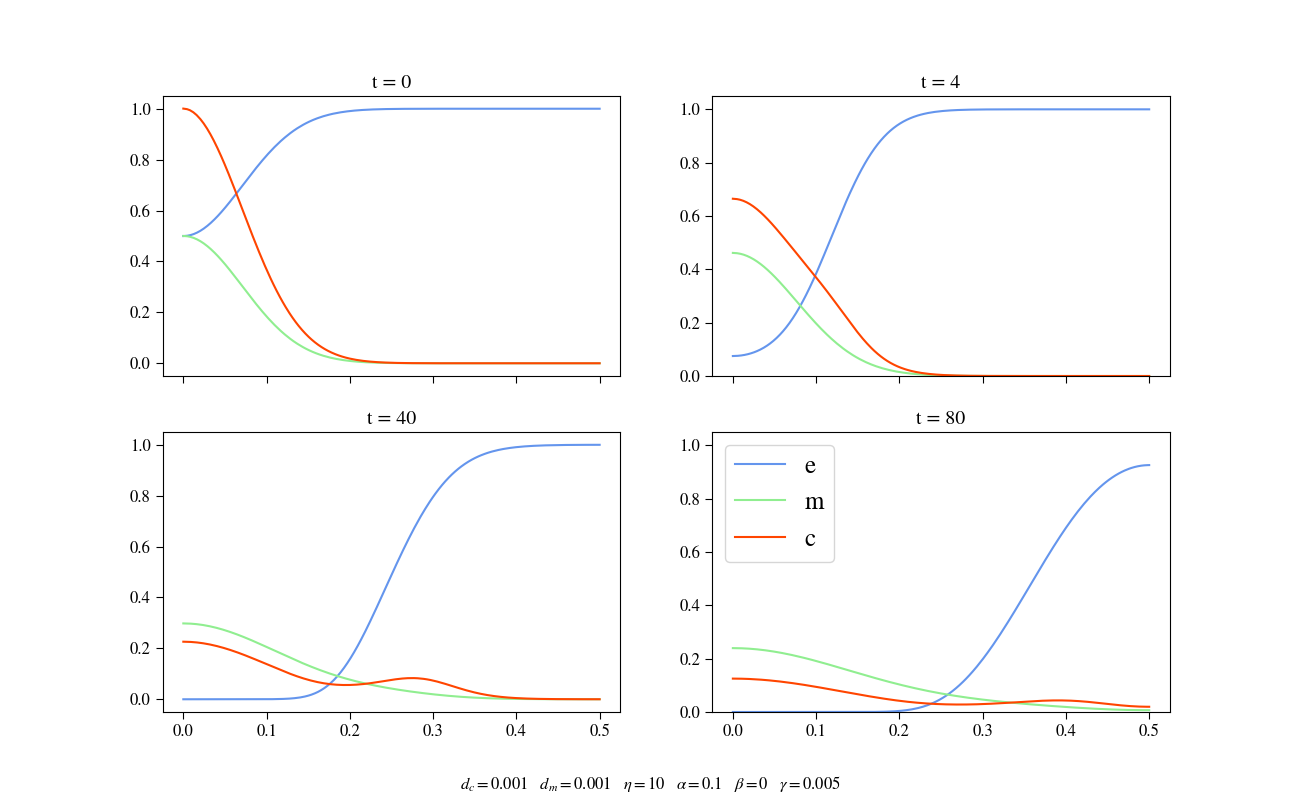
\includegraphics[width=\textwidth]{resources/images/2D_1e-3_1e-3_1e-3_10_0.1_0_0.005_1e-2_10_plot.png}
    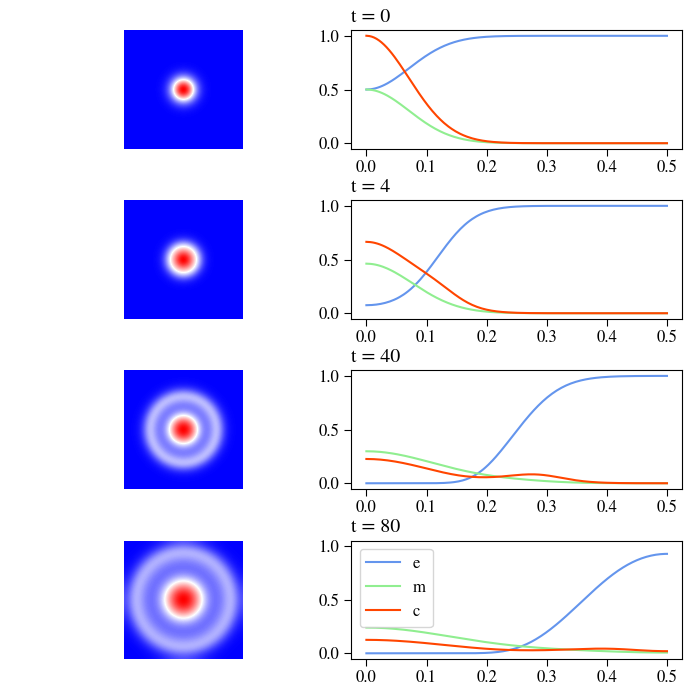
\includegraphics[width=0.7\textwidth]{resources/images/first_replication_results.png}
    \caption{Images on left side 2D plots of the experiment, images on right side results produced by applying plot over line tool}
    \label{fig:2D_1e-3_1e-3_1e-3_10_0.1_0_0.005}
\end{figure}

We therefore used the same parameters as in Anderson et al.s first one dimensional experiment with the values; $d_c = 0.001, d_m = 0.001, \gamma = 0.005, \eta = 10, \alpha = 0.1, \beta = 0, \mu_1 = 0, \mu_2 = 0$. Figure~\ref{fig:2D_1e-3_1e-3_1e-3_10_0.1_0_0.005} shows these results for four different points in time. Since our experiments are preformed in two dimensions you can see on the left side the two dimensional plots of the tumour cell density and on the right side you can see plots produced by applying the Plot Over Line tool confiugrated like described in the method section, where there is not only the tumour cell density visible but also the matrix decaying enzyme concentration and the extra cellular matrix concentration. We choose these points in time, because we used a different timescale than Anderson et al. and as you will later see, our time points capture the effects that can be observed studying their results quite well, which implies that for every time step Anderson et al. did we had to do 4. The problem with the two diemnsional plots is that as you can see overlazing the different variables of tumour cell density, MDE concentration and ECM concentration, makes the plots unreadable, so you can only show one at a time, additionally to this it is not possible to estimate values for c, e, m at different locations in space and time. These problems are solved using the plot over line tool, as you can see in the plots on the right side the curves for c, e, m are clearly distinguishable and we can estimate their values at locations. This is why for most experiments we resort to using the plot over line plots instead of full 2D simulation images, they make evaluating and comparing the respective experiments way easier and still capture for the most part all occuring effects. 
Starting from the inital values at $t=0$ we see that after four time steps a very small unevenness has formed for the tumour cell density at $x\approx 0.1$. Diffusion and Haptotaxis have stretched the curve for the tumour cells as did diffusion for the MDEs. The ECM has clearly been decayed at the origin.
The next image shows the simulation after 40 timesteps; we see that the unevenness of the tumour cell concentration of the previous point in time has been propagated to form a small hill at the leading edge of the tumour cells invading the surrounding tissue, at $x\approx 0.28$, this effect is due to the haptotatic influence, which pulls the tumour cells further into the accessible area towards the gradient of c grad e, creating a seperation for the tumour cell density, where the other part is still oriented towards the origin. MDEs also continued their diffusion into the area, decaying the ECM in their wake, decreasing them further. 
In the last image, after 80 simulation time steps, we see that as well the hill that has formed at the leading edge of the tumour cells as well as the concentration of tumour cells at the origin, have continued flattenting and taking on a constant concentration throughout space, though we can still clearly distinguish both areas. If we were to look at the simulation at later points in time, this curve will flatten even more, since with more time the ECM will be decayed and therefore the haptotactic flux coefficient $\gamma$ will lose its influence, leaving the movement of the cells to diffusion only. The curve for the MDEs has also flattened, yet not as strongly as the tumour cells concentration and as the observed before the ECM decayed where the MDEs were previously. Thez will continue to do so, decaying the ECM and their concentration over time will increase due to no limiting factors in this experiment and on-going production contributed by the tumour cells c.\newline
Comparing \ref{fig:2D_1e-3_1e-3_1e-3_10_0.1_0_0.005} to figure 1 in \cite{anderson_mathematical_2000}, we can see major differences. The first image showing $t=0$ looks the same, which confirms that both experiments start with the same initial values condition. In the images showing the simulation at the second time checkpoint we see that though the tumour concentration and ECM density values are approximately the same, the MDE concentration is slightly lower in our experiment, which will get more pregnant in the later images. The unevenness having formed at the leading edge of the tumour cell concentration also looks to be slightly smaller. The differences in the third image are more striking, both $c$ and $m$ have considerably lower concentrations, yet the ECM value looks to in line. In our case the diffusion of the tumour cells into the tissue also seems to happen a littel bit too fast. The last time checkpoints strengthens our findings, showing the same behaviour with ECM being approximately the same, tumour cell density and MDE concentration being clearly lower in our experiment and invasion of tissue happening too fast, leaving the lump at the origin $x=0$ too small. \newline 
This first of all confirms the initial supposition that with changing the dimension for the simulations the results also vary. We will now adjust the parameters iteratively to make the results using two dimensions mimick the results from Anderson et. al as closely as possible. For this we will start with varying the MDE production coefficient $\alpha$, to get higher concentration values, and also change the diffusion and haptotaxis terms of the tumour cells $d_c$ and  $\gamma$, to adjust the motitlity of the tumour cells and therefore also influence the invasion speed of them into the surrouding tissue.
\begin{figure}[h!]
    \centering
    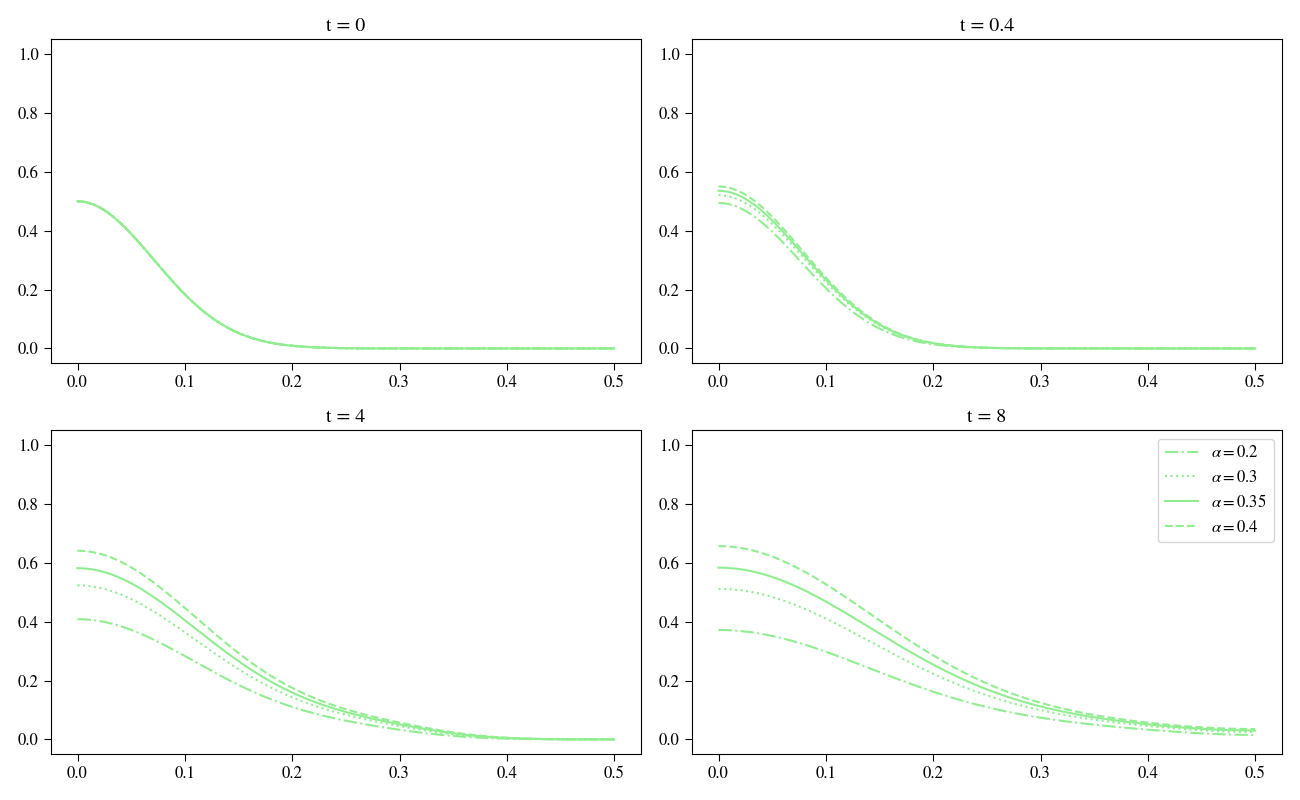
\includegraphics[width=0.8\textwidth]{resources/images/alpha_comparison.png}
    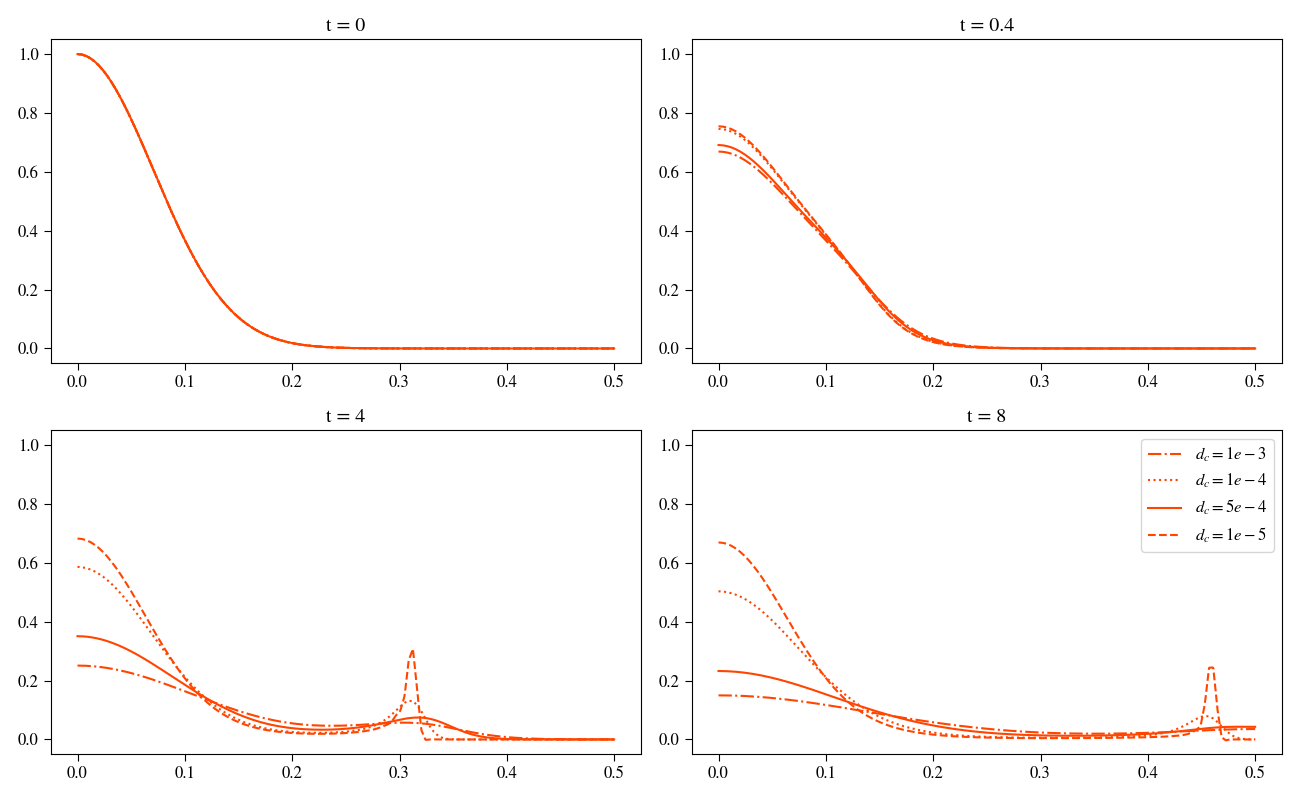
\includegraphics[width=0.8\textwidth]{resources/images/dc_comparison.png}
    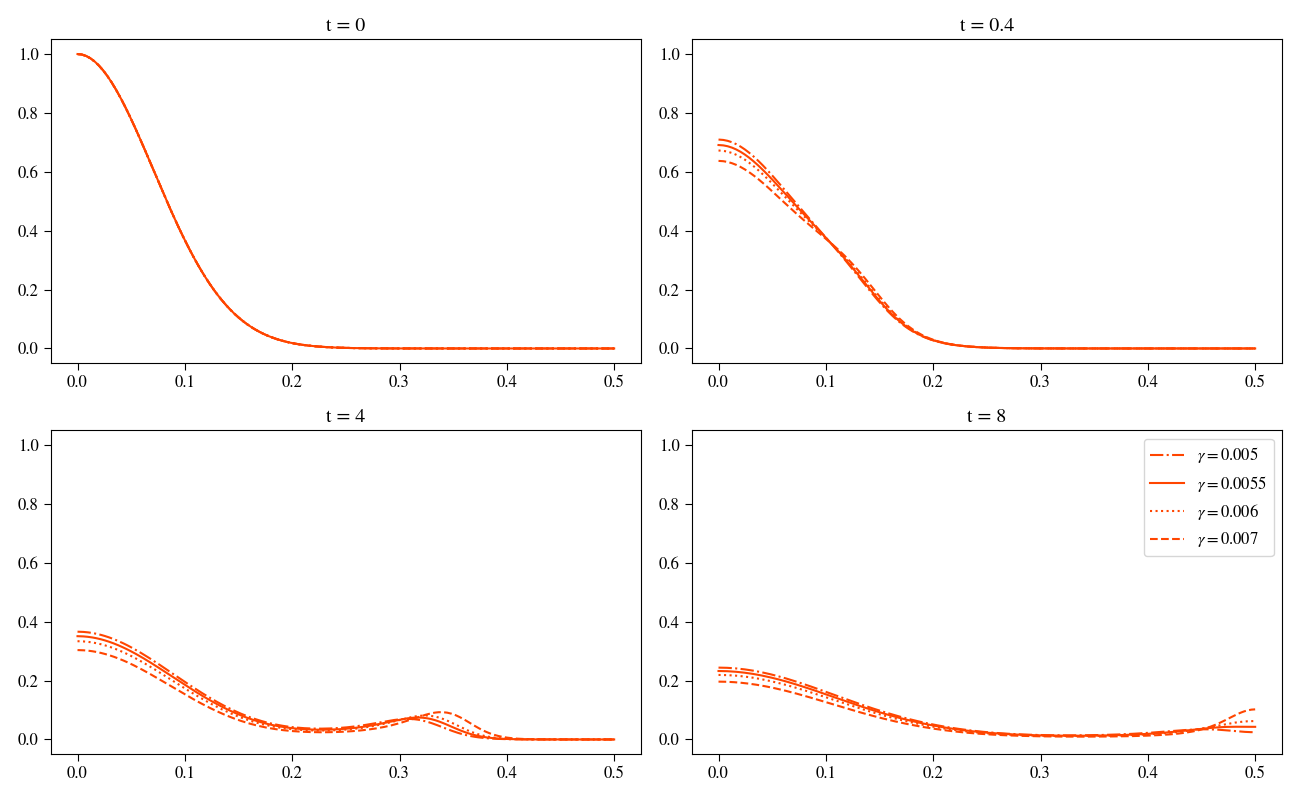
\includegraphics[width=0.8\textwidth]{resources/images/gamma_comparison.png}
    \caption{Caption}
    \label{fig:replication_comparison}
\end{figure}


Figure~\ref{fig:replication_comparison} shows a comparison of the parameters $\alpha$, $d_c$ and $\gamma$ have on a specific curve. Comparing different values for $\alpha$ and their effect on the curve of the MDE concentration, shows that, especially looking at the later points in time $t=4$ and $t=8$, with values for $\alpha$ between $0.3$ and $0.4$ we will get a good approximation. The values of the original paper for the MDEs are for $t=4$ $m(0)=0.6$ and at $t=8$ $m(0)=0.7$. Fine tuning this parameter led us to $\alpha=0.35645$.\newline 
Looking at $d_c$ we chose a value of $d_c=5e-4$. Using higher values for this parameter will result in numerical instability and results that are not useable. For $\gamma$ we made a slight adjustment upwards to $\gamma=0.0055$ to have a little bit more pull on the tumour cells outward, to match the invasion speed observed in the original paper. This yields results where the small hill at the leading edge of the tumour cell concentration in the latter two points in time is a higher values for $x$, yet not as steep as for example $\gamma = 0.007$. \newline

\begin{figure}[h]
    \centering
    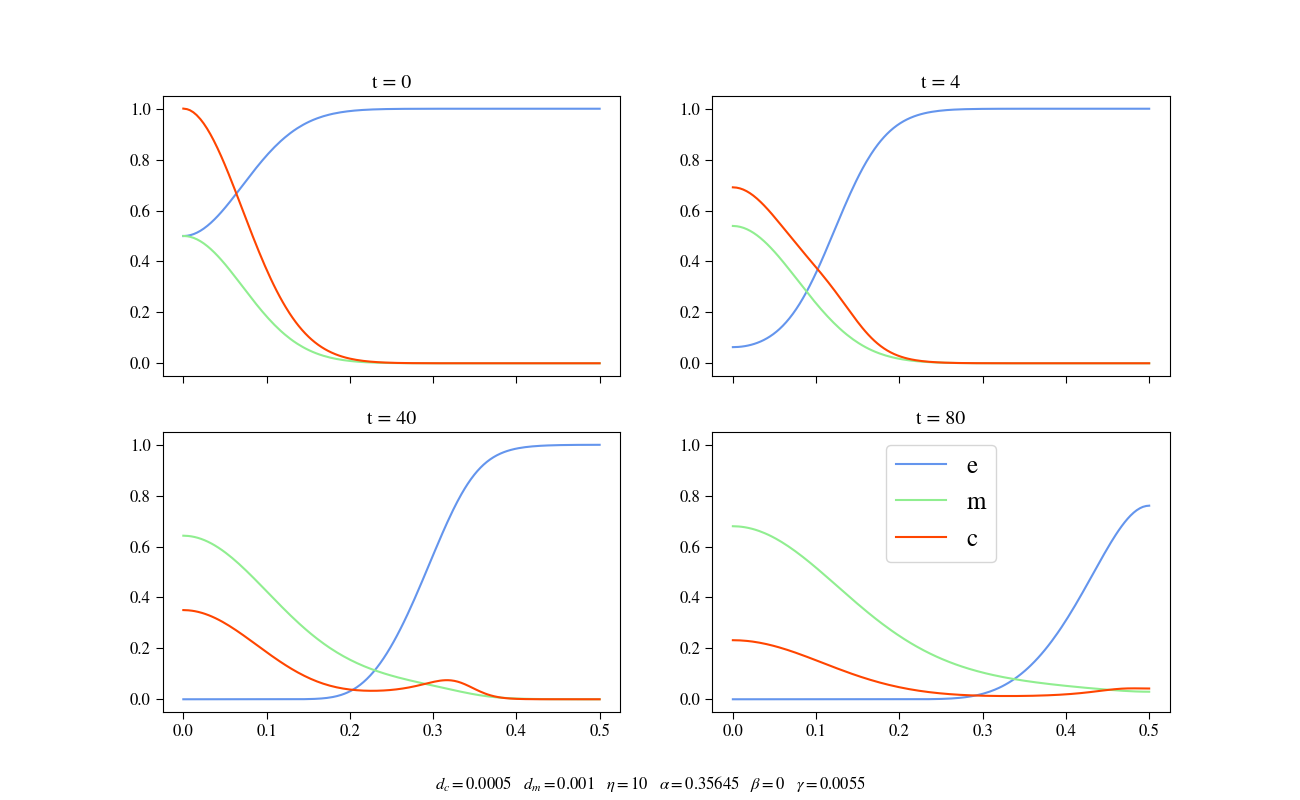
\includegraphics[width=\textwidth]{resources/images/basecase_without_proliferation.png}
    \label{fig:basecase_without_proliferation}
\end{figure}

These adjustments leave with the final configuration for replicating the system with the curves in figure~\ref{fig:basecase_without_proliferation} and the parameter settings also seen in the same figure.
Slightly adjusting the haptotatic flux to $\gamma=0.0055$ yields the following results, seen in figure~\ref{fig:fig:basecase_without_proliferation} comparing our final version with the original one we can see that in the second point in time, at $t=4$ in our case, the values of the three curves at the $x=0$ are nearly the same. In the original experiment the bump in the curve for the tumour concentration looks more pregnant, but this is only due to the fact, that this experiment was most likely done on the unit line, not the unit cube, it also seems that they have done a rescaling of the x-axis. The two later points in time confirm the similarity with having also nealy the same values for the three curves at $x=0$ but also their respective propagations in time look to be in line with the original experiment. 



\subsubsection{Parameter Analysis}
From the replicated results shown in figures~\ref{fig:2D_5e-4_1e-3_1e-3_10_0.35645_0_0.0055}, we saw that if we variate certain parameters the results also vary strongly. Therefore we are now going to have a look at how changing one parameter affects the output of the whole system. For this we assume the parameter values of the replicated results to be our set of baseline parameters, from there in each experiment only one parameter is changed. 
\subsubsection*{$d_c$ Variation}
The parameter analysed in this section describes the diffusion of the tumour cells and is integrated into the equations as being dependent on the laplacian of the tumour cells $\Delta c = (\frac{\partial^2 c}{\partial x^2} + \frac{\partial^2 c}{\partial y^2} + \frac{\partial^2 c}{\partial z^2})$. Leaving out the proliferation term our equation for $\frac{\partial c}{\partial t}$ also depends on $\gamma$ a coefficient for the haptotatic flux. The mathematical intuition is that if we will decrease $d_c$ we will see the effects of $\gamma$ taking over the simulation results for the $c$ curve, meaning that the tumour cells are more likely to drift outward and let themselves be pulled by the ECM concentration $e$, due to haptotaxis, leaving ony a little concentration at the center $x=0$, creating a bigger hill on the leading edge of the tumour concentration (below where $c \nabla e$ will be highest). On the other hand if we increase $d_c$ the effects of haptotaxis will diminish, the tumour cells will be subject to bigger diffusion pulling them more evenly into the tissue, there will be less of a leading hill being pulled outwards, since the diffusion will happen too fast, making this effect irrelevant. 
\begin{figure}[h]
    \centering
    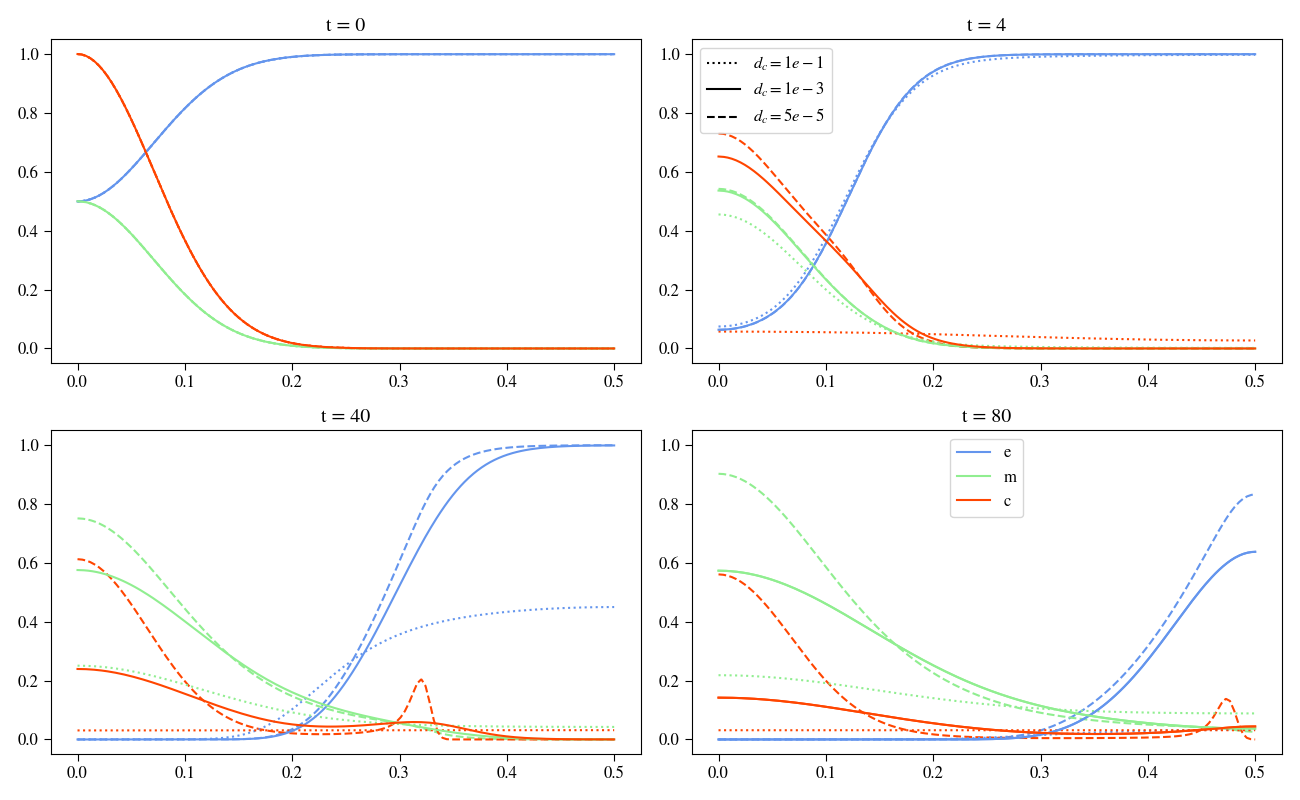
\includegraphics[width=\textwidth]{resources/images/dc_variation.png}
    \caption{Plots show results for varying $d_c$ whilst keeping the other parameters constant, in the images you can see the effects of $d_c=5e-5$ in the dashed curve, $d_c=1e-1$ in the dotted curve and $d_c=5e-4$ in the solid line.}
    \label{fig:dc_comparison}
\end{figure}
Looking at both experiments in figure~\ref{fig:dc_comparison}, we can see these assumptions confirmed. The smaller $d_c$ gets the higher the influence of $\gamma$ will be and vice versa. Considering the red curves, the tumour cell density, after $t=4$ timesteps the dashed curve, describing $d_c=1e-5$, takes on a value a little higher than for the basecase of the solid curve with $d_c=5e-4$ whilst the dotted curve, showing the results for $d_c=1e-1$, has already taken on a near constant concentration throughout space. This shows that the higher the values for $d_c$ are the faster the diffusion spreading throughout space will be, where for the solid and dashed line we can see small effects of haptotaxis in the second image, nothing of this is visible for the dotted line, where the diffusion effects completly cover up the effects of haptotaxis. For the MDE concentration we can observe that with rising values for $d_c$ they also spread faster throughotu space, this is first due to influece of the current $c$ density on the motility of the MDEs and also due to the production term, meaning with faster spread throughout space we will get more even prodution of MDEs. The effect on the ECM concentration varying $d_c$ seems to be little at stage. 
Looking at the next point time at $t=40$ we can see that the differences in the curves observed previously have intensified, with examining the tumour cell concentration, yielding now completly different results. The dotted curve has not visbily changed and while the solid curve describes the base case, we can see for the dashed curve that as above mentioned here the effects of haptotaxis, with a very pointy peak at the leading edge of the tumour cells. The other two curves differ also very visibly here, showing big variation MDE and ECM concentration. The MDEs diffuse fasater throughout space the higher $d_c$ is, with the dotted curve having flatted more than the other two, where the dashed curve has the highest concentration of MDEs at the origin still. This faster spreading of tumour cells and MDEs takes effect on the ECM, showing that the ECM for the dotted curve has clearly faster decayed than the other two, though for them we can see like for the MDEs visible differences considering degradation. 
In the last image we can see another amplification of the previous mentioned effects, for the dotted curves, $d_c=1e-1$, they seem to have taken constant concentrations in space, except the green curve for the MDEs which is till higher around the origin than in outer regions, the red curve descring the tumour cells has again not changed staying constant and the ECM concentration has also been decgraded towards zero every in space. The red dashed curve shows that the tumour cells density has two clear maxima in space one at the origin and one at the leading edge, whereas the solid curve is a lot more evenly distributed throughout space. Here you can also see that the red dashed curve takes on negative values, which indicate numerical instabilities, which will only increase decreasing $d_c$. These issues are due to the nature of the solver, where both factors influcencing $c$, $d_c$ and $\gamma$ need to be in a certain range to produces reasonable results, since negative values for the tumour cell density does not make any sense. The MDE concentration is as expected higher around the origin for the lower $d_c$ values, this is due to the tumour cells also staying rather around the origin for this experiment and therefore producing more MDEs at this location in space. It is interesting to see that both effects of $c$ and $m$ comparing the dasehd and solid curves seem to have little effect on the ECM concentration, but as we saw in the third image only a little concentraion of MDEs is needed to efficiently decrease the ECM, this shows that the ECM degradation process happens so fast that minor diffrences in the MDE concentration have little effect on it and also as we can see that the major differences in the MDE curve are located around the origin, these differences seem to decrease with increasing distance.
These comparsion verifies that $d_c$ has a rather impactful influence of the system, espeically considering that the $d_c$ values of the dashed and solid curves are only seperated by a distance of $5e5$. Increasing $d_c$ results in faster diffusion and also faster spreading throughout space, but also with faster degradation of the ECM and invasion of MDE of the area.

\begin{comment}
In the first four images we can see the results for $d_c=1e-5=0.00005$, while in the it looks mostly normal with little of the secession building at the leading edge, we can see that in the third image, this secession has not only seperated itself from the main lump of cells, but has also developed a sharp peak, which would have negative consequence regarding the differentiability of the $c$ curve. In the fourth image this behaviour is even more extreme and looking closely at this simulation in ParaView, the values for $c$ take on a negative sign, which from a biological perspective does not make any sense since there can't be less than zero cells at a position in space. This indicates a numerical instability, which decreasing $d_c$ even furhter also resulted in oscilations in the $c$ curve and even more negative values for the tumour cells. This instability is due to numercial model used, which only yields useful results if $\gamma$ and $d_c$ are in a certain range. This could be a point for further investigation, inspecting how the results change if $\gamma$ and $d_c$ are both varied at the same time and finding this range $\gamma$ and $d_c$ need to be in to make sense. However looking at the other two curves $e$ and $m$ we can see that they still make sense, especially also in the first experiment with $d_c=1e-5$, $m$ at the start following where $c$ was high, exceeding $c$ at some point due to the production factor $\alpha$ and $e$ decaying where the MDEs have higher values. Interesting is that having high values for the diffusion coefficient the concentration is faster evenly distributed in space, which indicates a higher invasion pace, which in turn makes the degradation of $e$ happen a lot faster, though the MDEs have taken on a near constant niveau throughout space. This also indicates, that we don't need to have a visibly higher concentration of $m$ to degrade the ECM. 
\end{comment}

\subsubsection*{$\gamma$ Variation}
Inspecting the effects of $\gamma$ we can assume the same as for $d_c$ if we select higher values for $\gamma$ the effects of haptotaxis, pulling the tumour cells into the tissue faster, leaving no cells at the origin, taking lower values for $\gamma$, the diffusion will be superior factor for the tumour cell motility, which will result in no secession at the leading edge of the tumour cells.
\begin{figure}[h]
    \centering
    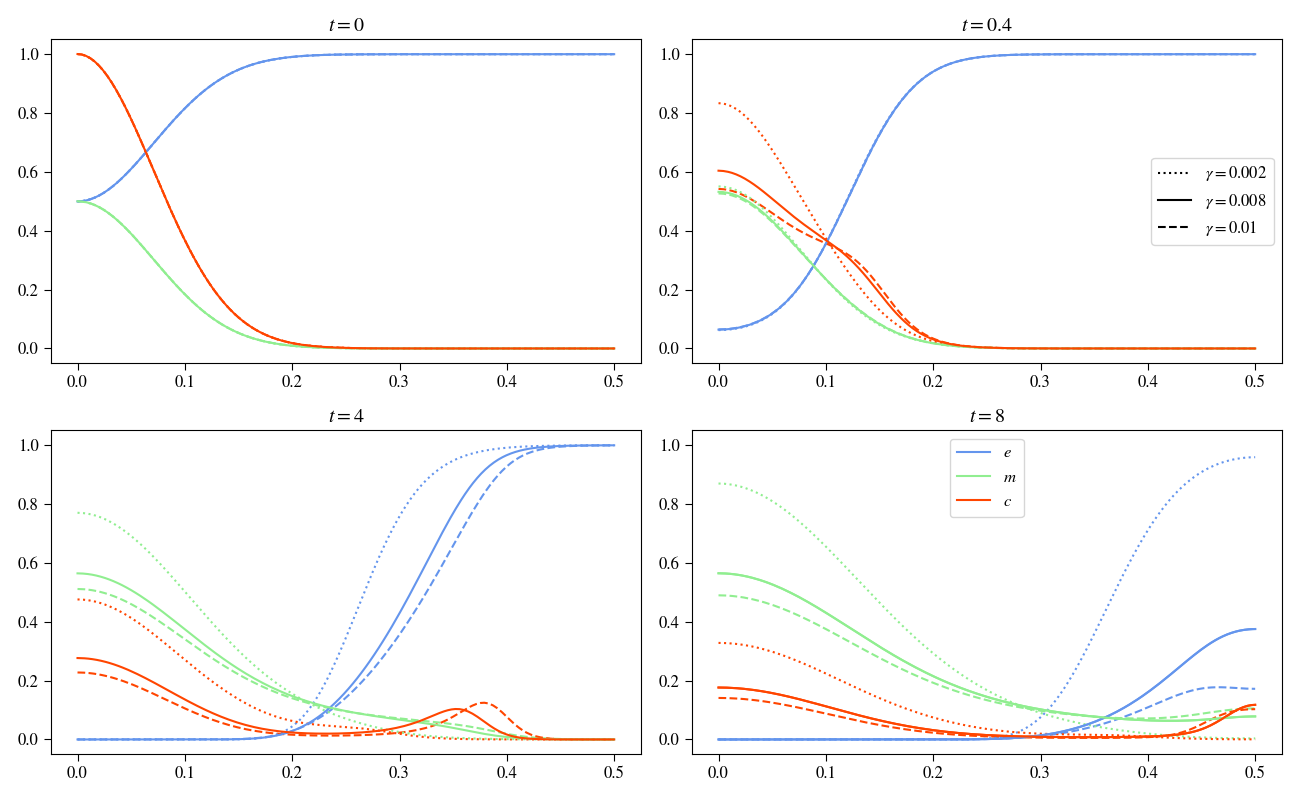
\includegraphics[width=\textwidth]{resources/images/gamma_variation.png}
    \caption{Plots show results for varying $\gamma$ whilst keeping the other parameters constant, in the images you can see the effects of $\gamma=0.01$ in the dashed curve, $\gamma=0.002$ in the dotted curve and $\gamma=0.008$ in the solid line.}
    \label{fig:gamma_variation}
\end{figure}
The experiments, described in figure\ref{fig:gamma_variation} verify the expected behaviour. After $t=4$ the solid and dashed red curves, indicating tumour concentration for the higher values for $\gamma$, have already built a lump that will in the later points in time form a secession, here we can already see that the dasehd line with the highest value for $\gamma$ has formed a larger lump than the curve for $\gamma=0.008$.The tumour density curve for $\gamma=0.002$ does not show such bevahiour. The curves for the MDE and ECM concentration still overlap at this point in time. The next image showing the simulation after $t=40$ timesteps shows that changing $\gamma$ affects also the other curves. Whilst the tumour concentration for the values of $0.008$ and $0.01$ differ slightly by the amount of density thath is left at the origin and the distance they have already invaded the surrouding tissue, the curve for the value $\gamma=0.002$ does not even show a leading edge here that is being pulled by haptotaxis into the tissue, yet it has the highest density at the origin for the $c$ curves. We can also see that with increasing $\gamma$ the invasion speed also increases. 
For the MDE curve we observe that it is still hihgest at the origin for the curves of $c$ that have lower values for $\gamma$, this only makes sense since the tumour cells produce the MDEs. For the ECM concentration we see similiar behaviour as for the MDEs, with increasing $\gamma$, the ECM is also faster decayed, again this also makes sense, since for higher values the $c$ curve curve has invaded faster and has therefore established more MDEs at farther locations away from the origin decaying the ECM.
The last image at $t=80$ confirms the observations from the previous points in time; the higher $\gamma$ the faster the invasion pace of the tumour cells and the MDEs and therefore the faster the degradation of the ECM. 
When we now take a step further and increase $\gamma$ by one potence, to $\gamma=0.1$, we can observe that the invasion pace, has gotten so high, that before finishing the simulation at $t=80$ the tumour cells have not only invaded completely up to the border regions but have also been pulled back towards the origin upon getting reflected at the border of the unit square and also since degradation of the ECM has not kept up with the invasion pace of the tumour cells,we are left with a situation where the tumour cells have spread further than the ECM and are now being pulled back inwards toward the origin again, this can be seen in figure \ref{fig:gamma_2D_plot}. After already $t=20$ the tumour cells shown on the left side in this figure they have almost reached the border, looking at the ECM at this point in time we see that the highest concentration is now in the corners of the unit square. so this is where the haptotaxis is going to pull the tumour cells, this behaviour is not anymore radially symmetrical. We see in the next point in time at $t=30$ that the tumour cells do exactly this moving into the corners of the plot. Figure \ref{fig:gamma_pol_comparison} underlines this abondoning of radial symmetry, on the left side we see the plot over line configuration we used until now, the left side shows a plot over line configuration from the origin to one of the corner. After $t=20$ the images on left side imply that the tumour cells get slowly pulled back in after being reflected on the boreder, yet with a lower density, on the right side we see that tumour cells are still getting pushed outwards into regions where there is still the most ECM. In figuer \ref{fig:gamma_alt_plot} you can see the plot over line results using this alternative configuration. Up until $t=20$ everything looks like in the normal plot over line results. After this keeps going unitl hitting the border and getting reflected at $x=0.7$ which is reached between the latter two points in time. Upon getting reflected you can also see that the concentration along this line increases visibly, this is due to the tumour cells moving into the corners that have reached their borders earlier in time. As you can see this also influences the MDE and ECM concentration, with curves that are not montone since they could keep up the pace of the tumour cells invasion speed. Whilst the ECM in regions at $x=0.25$ have not decayed at $t=60$ they from a single maxima at this point, the MDEs that have been produced at the origin are at this point in time are at the same point $x=0.25$ joined by the MDEs coming from the border regions where the tumour cells there have produced them.
Where in all of the other experiments for varying $\gamma$ the tumour cells invaded at such a pace, that the produced MDE concentration in their wake was sufficiently high to degrade the ECMs to not pull the tumour cells back to the remaining ECMs later and produce montone results for both ECM and MDE concentration.
Though the intuition is met that with increasing $\gamma$ the invasion pace of the tumour cells and matrix decaying enzymes also rises, we get unexpected behaviour with the tumour cells invasion being so fast that they get reflected at the border of the unit cube and pulled into the corners and from there back in by not decayed ECM. Further increasing $\gamma$ will only increases this behaviour and make this osicilating process even faster.

\begin{figure}[h]
    \centering
    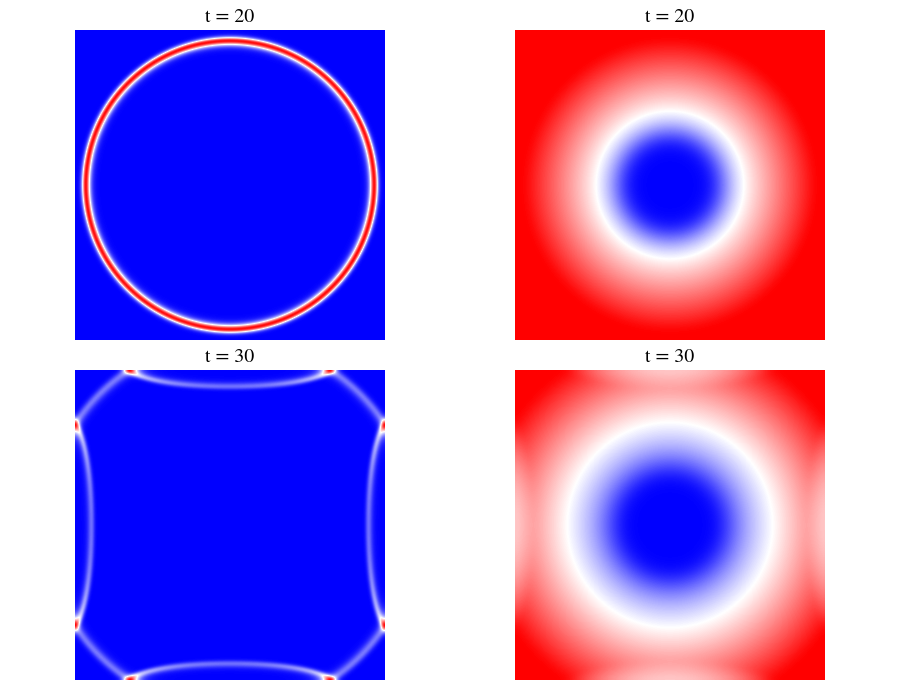
\includegraphics[width=0.9\textwidth]{resources/images/2D_plot.png}
    \caption{2D plot of variation}
    \label{fig:gamma_2D_plot}
\end{figure}
\begin{figure}[h]
    \centering
    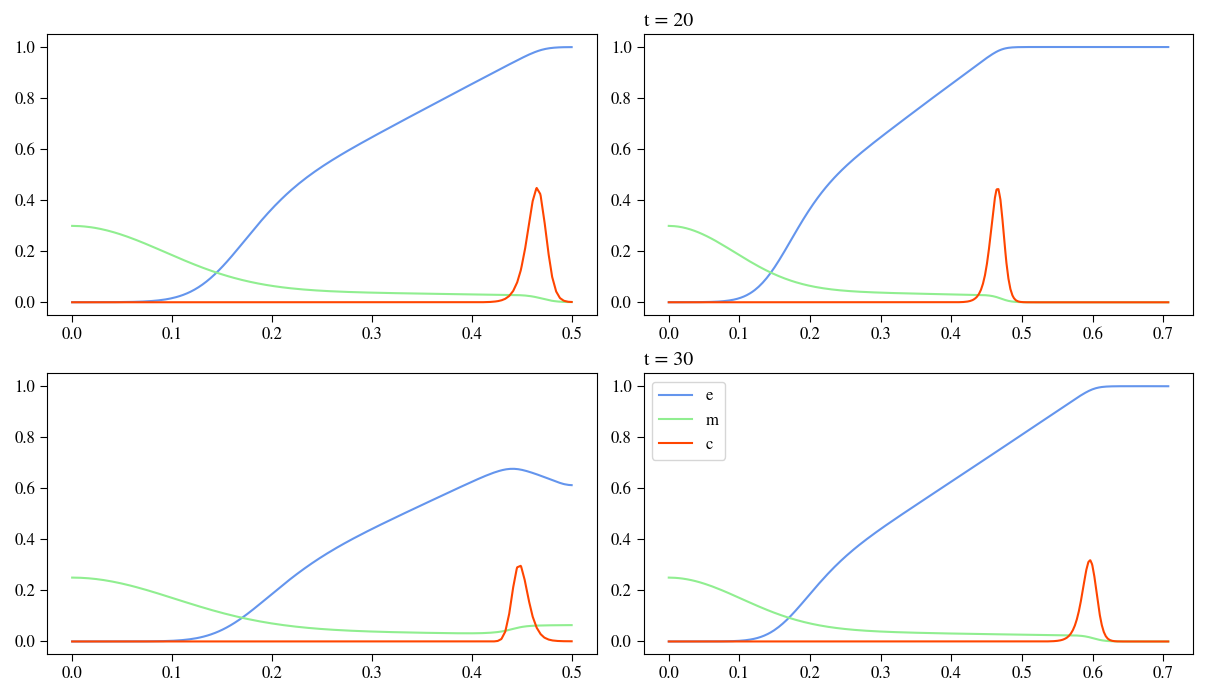
\includegraphics[width=\textwidth]{resources/images/pol_comparison.png}
    \caption{Plot OVer Line Comparison Gamma}
    \label{fig:gamma_pol_comparison}
\end{figure}
\begin{figure}[h]
    \centering
    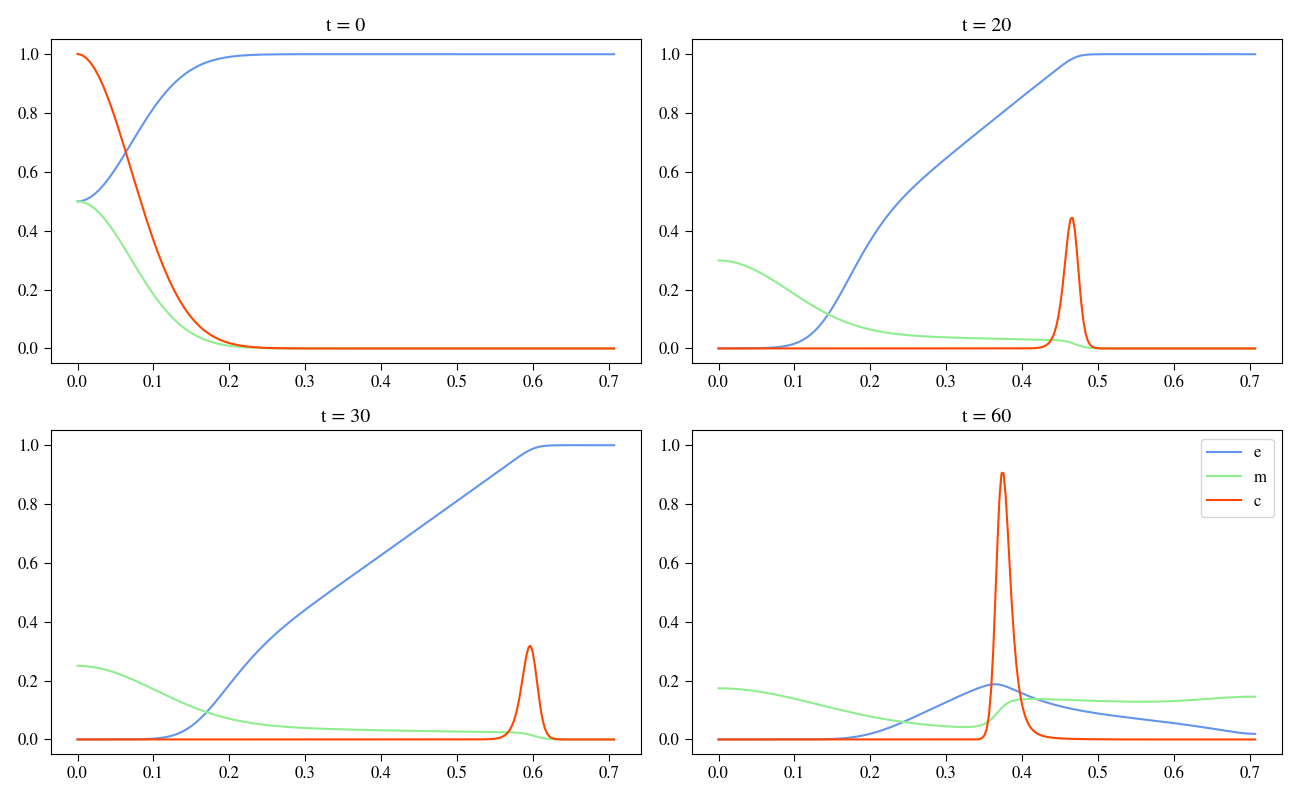
\includegraphics[width=\textwidth]{resources/images/gamma_alt_pol.png}
    \caption{gamma alternative plot over line}
    \label{fig:gamma_alt_pol}
\end{figure}

\subsubsection*{$\eta$ Variation}
\begin{figure}[h]
    \centering
    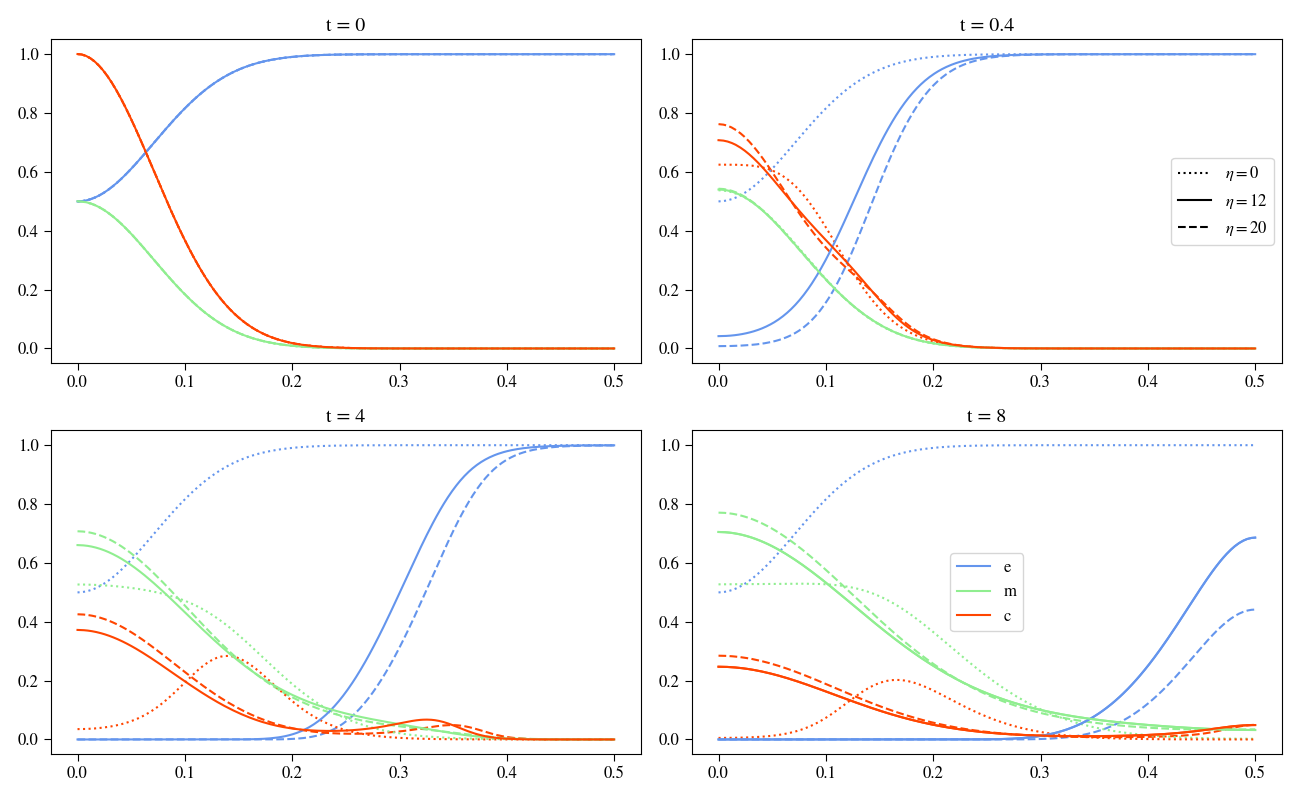
\includegraphics[width=\textwidth]{resources/images/eta_variation.png}
    \caption{Plots show results for varying $\eta$ whilst keeping the other parameters constant, in the images you can see the effects of $\eta=20$ in the dashed curve, $\eta=0$ in the dotted curve and $\eta=12$ in the solid line.}
    \label{fig:eta_variation}
\end{figure}
The parameter $\eta$ influences the degrading of the ECM, which happens faster for higher $\eta$ coefficients in regions where both MDE and ECM concentration are high. Varying this parameter may have a high impact of curves for $c$ as well, because the gradient of the ECM is a deciding factor for the effects of haptotaxis on the tumour cells, thus increasing the degradation may cause a faster shift of the ECM outwards, therefore also pulling the tumour cells faster farther out, which in turn will affect also the MDE curve.\newline
Inspecting the images in figure~\ref{fig:eta_variation} we see those assumptions met. Across all images you can see that with $\eta=0$, the dotted curves, the curve describing the ECM concentration stays constant, $\frac{\partial e}{\partial t} = 0$, this causes the tumour cell density to create no hill at the leading edge invading the tissue, since the haptotatic effect of the pull of the ECM is limited to happen with a distance of $x=0.2$. At the two later points in time the tumour cells for the experiment with $\eta=0$ take on a distribution with only one maximum located beneath where the value for $\delta c (\delta e)$ is highest, due to this point not changing much, the curve for $c$ does neither. Due to the limited motitlity of the tumour cells they doe not invade the tissue at all. The curve for the MDEs also looks much different from the basecase, after increasing intially slightly at $t=4$, the curve curve interestingly does not increase over this limit of $0.528$, with the tumour cells invading the tissue the MDEs follow with their production as well. Since the maximum of $c$ does not drastically change after $t=80$ the curve for the MDE continues increasing in this region as well, though not as strongly since the tumour cells concentration also diffuses over time. 
The solid curve describing $\eta=12$ does not strongly differ from the base case, exhibiting the expected behaviour of a stem of cells splitting off the main bulk invading the tissue at a faster rate and after $t=80$ having invaded the outer regions of the tissue as well. The curves for the MDEs and ECM follow the description of the basecase experiment. 
Increasing $\eta$ to $20$, the dashed line, the behaviour change is not so drastic comparing it to $\eta=12$. Thoug the degradation of the ECM happens twice as fast, the resulting accellerated invasion pace of the tumour cells, is not this pregnant. Interesting is that the hill at the leading edge of the tumour cells is though farther out also smaller than for the previous experiment, this might be due to the accellerated invasion pace, the tumour cells leading hill is also stretched farther. The remaining lump of tumour cells at the origin has also taken on a higher value than the experiment for the solid line, reason for this could be that with the faster degradation the effects of haptotaxis have a bigger influence on regions that are farther away from the origin, which will leave the remaining cells at the origin more subject to diffusion, because of the faster degradation the tumour cells at $x=0$ are a shorter time influenced by strong haptotatic pull, leaving more of them at the origin. Looking at the ECM concentration it has after $t=80$ as expected more decreased than previous experiments varying $\eta$. The MDE concentration has at the origin where the tumour cell concentration is higher for $\eta=20$ than for $\eta=12$ also a higher concentration, moving farther out we can also see that in those regions it is slightly lower than for the experiment with $\eta=12$, this only makes sense, since there the tumour cell density, producing the MDEs is not as strong. 
Overall we can see that with increasing $\eta$ the ECM degrading process is accellerated and also the invasion pace, with the tumour cells we can observe that due to faster invasion the remaining cells at the origin have a higher concentration as for the basecase, yet the hill at the leading edge of the tumour cells is smaller and for the MDEs they mimick this behaviour with a larger concentration at the origin as the basecase though smaller concentration at the invasion edge of haptotaxis.

\subsubsection*{$d_m$ Variation}
\begin{figure}[h]
    \centering
    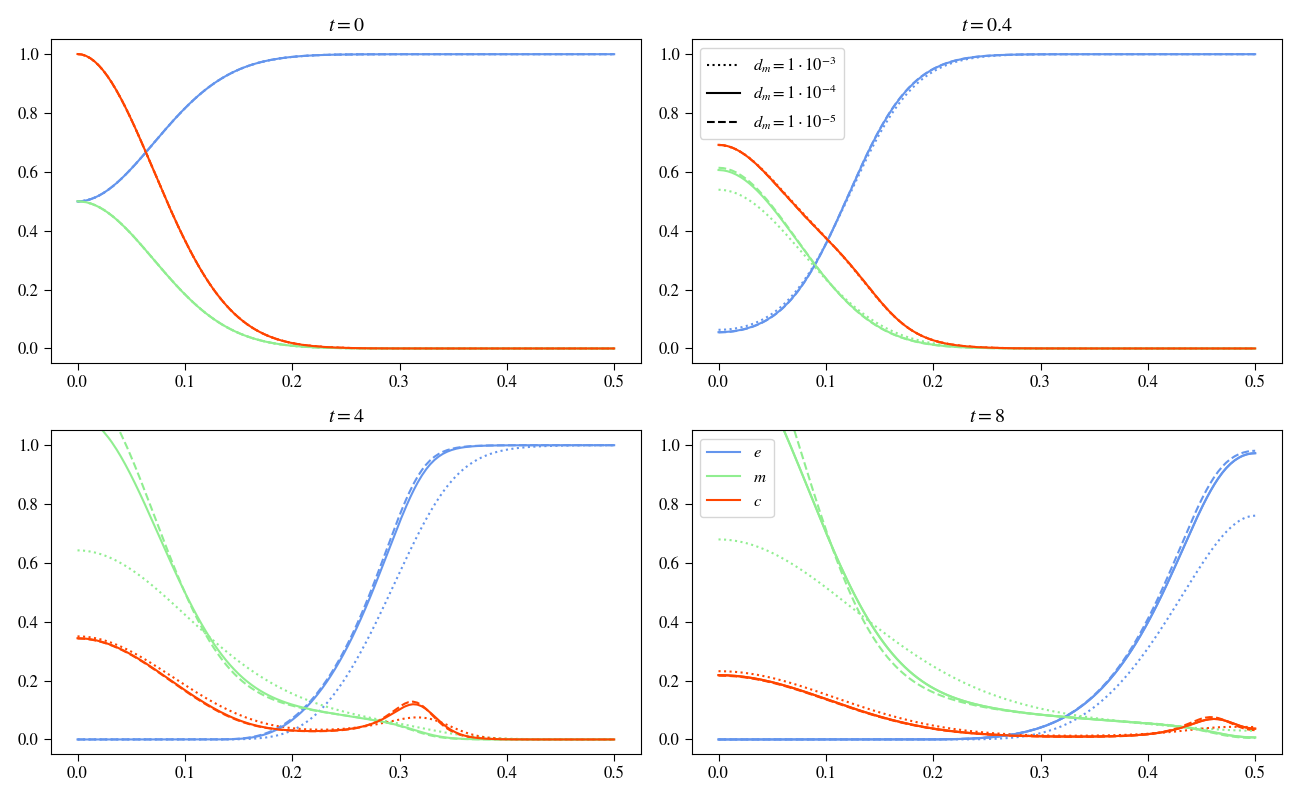
\includegraphics[width=\textwidth]{resources/images/dm_variation.png}
    \caption{Plots show results for varying $d_m$ whilst keeping the other parameters constant, in the images you can see the effects of $d_m=0.1$ in the dashed curve, $d_m=0$ in the dotted curve and $d_m=0.001$ in the solid line.}
    \label{fig:dm_variation}
\end{figure}
$d_m$ is the parameter describing the diffusion of the matrix degrading enzymes MDEs, it is influcenced by the laplacian of c, $\Delta c$. Looking at the equations we can expect with higher values for $d_m$ a faster degradation of $e$, since the MDEs can diffuse faster into the space and there isn't a high concentration of MDEs required to efficiently degrade the extra cellular matrix $e$. This will not neccessarily cause a faster invasion pace of $c$, because the ECM could be degraded more evenly and get degraded in such a way that we dont get two clearly distinctable niveaus of their concentration.
Inspecting the second image after $t=4$ we see that for $d_m=0$, the solid curve, there was no movement, the curve changex only due to the production of new MDEs contributing from the tumour cells. For $d_m=0.001$ we see that its dotted curve is slightly larger at the center but moving outward it surpasses the solid curve again, the diffusion happeining mainly toward the origin at this stage. The dashed curve shows $d_m=0.1$ and in this case the MDEs have already after four timesteps taken on a constan distribution throughout space. This influences both of the other dashed curves, the tumour cells get pulled out faster and the ECM degradation is more advanced for the other two cases. For them the curves for ECM and tumour cells look nearly identical.
The next point in time $t=40$ yields interesting results. The curve of the MDEs for the case of $d_m=0$ surpasses one for the first time in the region around $x=0$, due to no outward movement and the density of tumour cells at the origin, though as the dotted ECM curve $e$ shows the degradation happens slower than for the other two cases. Interestingly the tumour cells have developed a steeper hill at the leading edge of them invading the surrouding area, due to being exposed to strong haptotactic pull for a longer time. 
Looking at the dashed line experiment, $d_m = 0.1$ we observe that the concentration of the MDEs is still constant though it has visibly risen compared to the previous image, because the produced MDEs everywhere are being distributed evenly throughout space again. As mentioned above the ECM have degraded in such a way that there are no two niveaus of them clearly distinctable due to the MDEs being already everywhere in space. This causes the effects of haptotaxis to diminish, since $\nabla e$ is decreased and therefore the tumour cells don't experience a strong pull to invade the tissue around them, resulting in such a configuration that the dashed red curve is more evenly stretched along the x-axis.
In the last image at dimensionless time $t=80$ we can observe for the dotted lined experiment, $d_m=0$ the value of the MDEs has further risen at the origin, the ECM degrading was slower than the other two and the tumour cell density of this experiment is the only one that still has a hill at its leading edge due to haptotactic pull, with the highest gradient for $e$ at this point in time. The dashed curves for the MDEs conitinue to be constantly distributed throughout space, having again clearly risen compared to the previous point in time, the blue dashed curve for the ECM is constantly zero everywhere in space, which nullifies the effect of haptotaxis on the tumour cells, leaving them only to be influcenced by diffusion, causing an more even distribution of the tumour cells throughout the space. 
As we assumed initally with improved motitlity of the MDEs the degradation happens faster, but as we also suspected the invasion does not neccessarily happen faster. Due to the ECM being complelty degraded at the last point in time the tumour cell's motiltiy is only subject to diffusion of them, which is not sufficient at this point in time, to make them invaded the border regions of the area.
	

\subsubsection*{$\alpha$ Variation}
\begin{figure}[h]
    \centering
    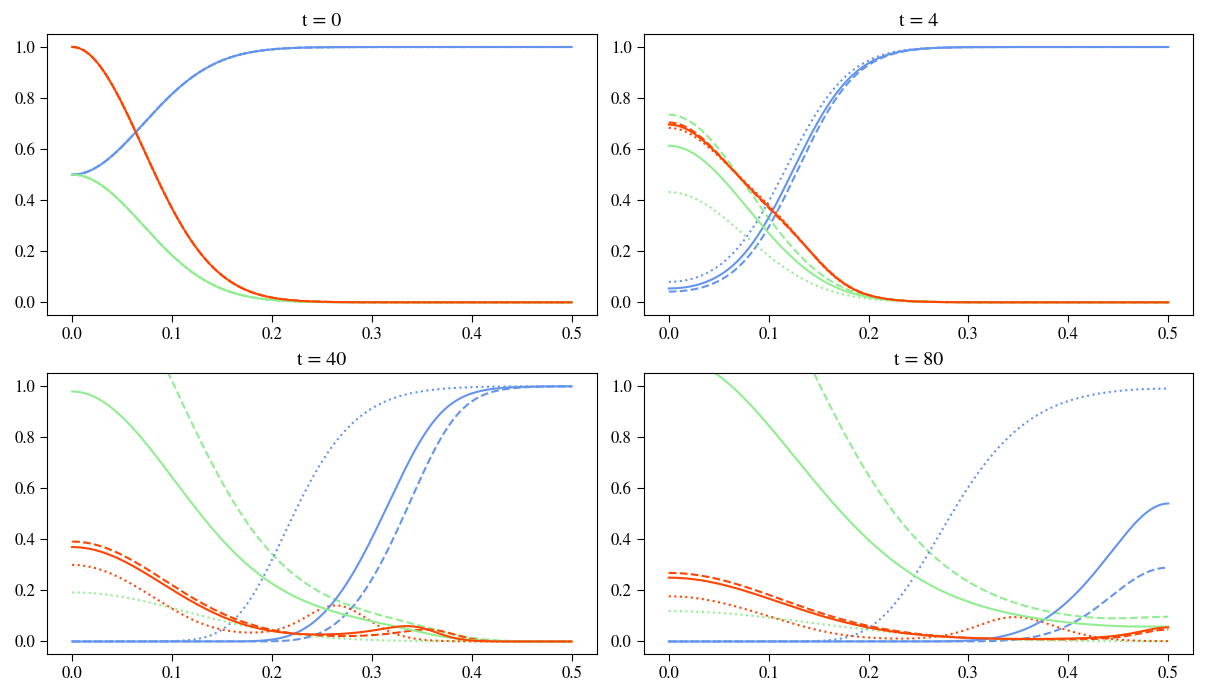
\includegraphics[width=\textwidth]{resources/images/alpha_variation.png}
    \caption{Plots show results for varying $\alpha$ whilst keeping the other parameters constant, in the images you can see the effects of $\alpha=1.0$ in the dashed curve, $\alpha=0$ in the dotted curve and $\alpha=0.6$ in the solid line.}
    \label{fig:alpha_variation}
\end{figure}
The parameter $\alpha$ influences how fast the tumour cells produce matrix decaying enzymes, looking at the system of equations it therefore depends on the concentration of tumour cells. Trying to replicate Anderson et al's experiment we already see how varying $\alpha$ affects the simulation results. Here we wil take a look at within the range of from $0.0$ to $1.0$. We can expect with growing $\alpha$ a higher concentration of MDEs which in turn will cause faster degrading of the ECM. Faster ECM degrading could mean increased invasion of the tumour cells. As we saw in the previous experiments varying $d_c$, the MDE concentration can take on values higher than one, we can also expect this here when $\alpha$ is sufficiently high.
In the second image, describing the experiments after $t=4$, we can see that the difference in the MDE curve for the different values of $\alpha$ is clear, the higher $\alpha$ the higher the concentration of the MDEs. The other curves seem not be affected as strong at this point in time though we can already see especially for th ECM concentration that the higher $\alpha$ the faster the degradation of the extra cellular matrix has already happened. The curve of the tumour cells looks almost identical for all values of $\alpha$, looking very closely we can see small deviations around $x=0$, here the previous trend is supported with higher values for $\alpha$ corresponding to also higher values for the tumour cell density. This is interesting since faster degradation as we saw varying $\eta$ results in faster invasion, but it can be explained, by the fact that with degradation happening at an increased pace, the tumour cells effect of haptotaxis also happens more strongly at regions farther away from the origin, stretching them farther out but also leaving a higher concentration at $x=0$.
The next point in time at $t=40$, shows the previous mentioned effects in an intensified way. Whilst for $\alpha=0$, dotted curves, the MDEs have no producing factor the curve flattens throughout space due to diffusion, never exceeding the value of $0.2$ for their concentration. For the ECM we see that though it has degraded visibly this happened at a slower rate than for the other experiments. The tumour cells have lowest density at the origin of the three variations, but it's hill at the leading edge has the highest volume, as explained above, due to slowed degradataion the tumour cells at the origin are a longer time subject to higher influences of haptotaxis pulling more of the cells into the surrounding tissue. The solid curves describing $\alpha = 0.6$ show that at this point in time they have almost reached a concentration of one at the center, which implies that in the following time steps the value here will exceed one. With the tumour cells have invaded farther out than in the experiment with $\alpha=0$ the ECM degradataion has also been happening faster.
Looking at the dotted lined experiment, indicating $\alpha=1.0$ the value of the MDEs at the origin has already exceeded one by far, with a value of $1,55$ at $x=0$, thus the degradation is faster, with a lower ECM curve and faster invaded tumour cell curve. 
In the last timestep we see that the MDE curve of both $\alpha=0.6$ and $\alpha=1.0$ have exceeded one. The dotted curve of the MDE shows that diffusion has distributed the MDE more evenly throughout space. At the border regions we see that the dotted curve is also the only one that has not yet degraded any ECM in this regions, whilst the dashed curve shows that there is only a little ECM concentration left to degrade. This is also shown in the curve of the tumour cells, whilst the dotted curve's peak is still somewhere around $x=0.35$ the other two curves indicate complete invasion of space. 
Our initial assumptions are correct with a faster degradation pace due to higher MDE concentration and therefore a faster invasion pace of the tumour cells. Whilst it makes from a numerical perspective sense that the concentration of MDEs can exceed one, it might make sense to introduce a finer grid or adapt the model in other ways, since judging from a continuous perspective it does not really make sense that at a certain point in space there are more than one entities, occupying this space. 

\subsubsection*{$\beta$ Variation}
\begin{figure}[h]
    \centering
    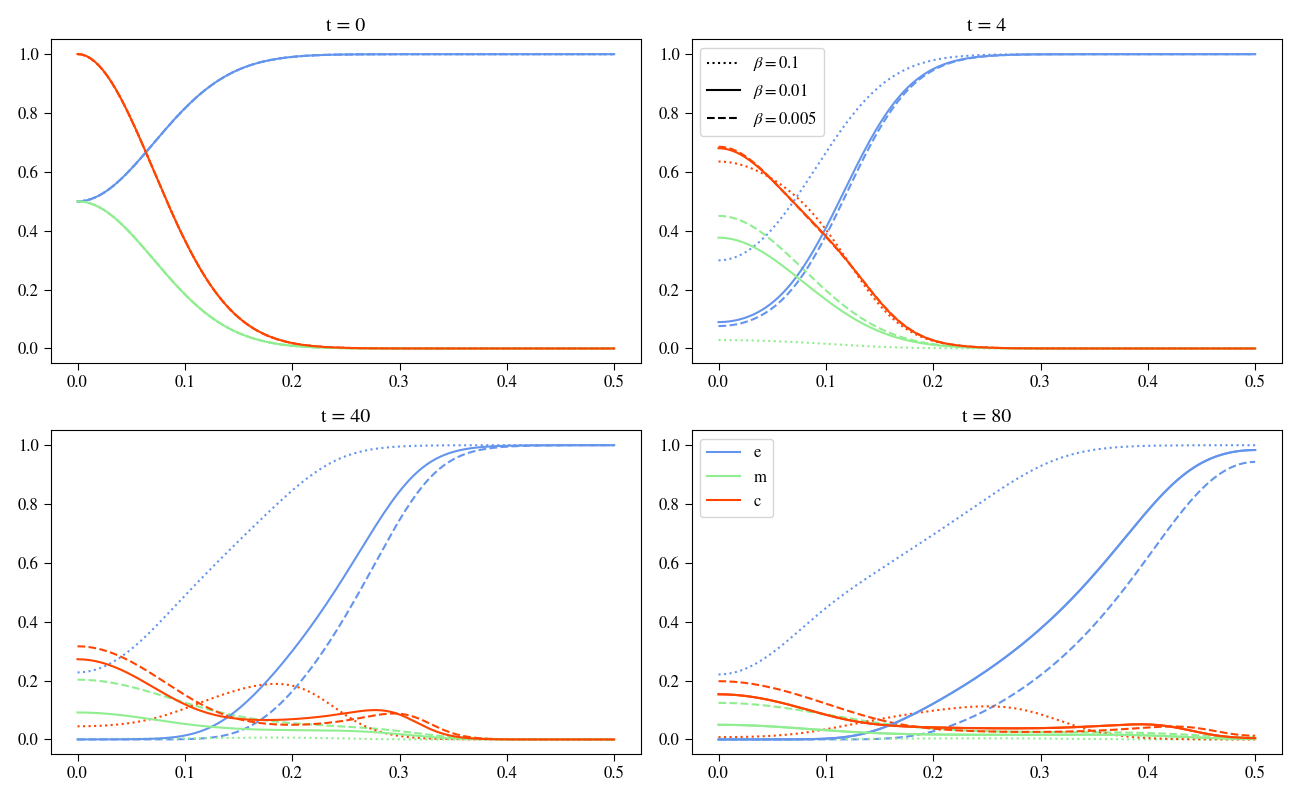
\includegraphics[width=\textwidth]{resources/images/beta_variation.png}
    \caption{Plots show results for varying $\beta$ whilst keeping the other parameters constant, in the images you can see the effects of $\beta=0.005$ in the dashed curve, $\beta=0.1$ in the dotted curve and $\beta=0.01$ in the solid line.}
    \label{fig:beta_variation}
\end{figure}

Looking at a variaton of $\beta$, in figure~\ref{fig:beta_variation} which is the parameter describing decay of the MDEs, we can assume that with varying $\beta$ the MDE curve will be lower, influcencing the ECM degrading process and therefore also the invasion pace. Since all previous experiments assumed a value of $\beta=0$ we are going to look for a value here that is neither too high to distort the whole simulation nor a value too low to have no effect on it. We first of all needed to determine a range in which to experiment. Starting with a range of values between $0.1$ and $1.0$, since this is the range $\alpha$ yields reasonable results in and $c$ and $m$ are in the same scale regarding their values, we counter-intuitively saw that those values were much too high. Even for $\beta=0.1$, shown in the dotted curve, the MDEs are almost completely decayed after only $t=4$, leaving only a small portion of MDEs at the origin due to the production from the tumour cells.
This makes the ECM degradation process visibly slower and makes the tumour cells a longer time subjected to high effects of haptotaxis, causing to only develop one hill, visible in the red dotted curve.
Looking at the different points in time we can see that though the dotted green MDE curve is nearly everywhere zero we see that degradation still happens visibly and due to the longer exposition on haptotaxis on bigger portions of tumour cells this one lump of cells is being pull through space.
Decreasing to $\beta=0.01$ we see that the for the solid lines in figure~\ref{fig:beta_variation} the MDE concentration takes on higher values througout the points in time. The tumour cells density show again a distinction between the effects of diffusion and haptotaxis, resulting in a two distinctly different lumps with different maxima and ECM degrading resembles most of the previous experiments, though the gradient here is not as steep especilly in the last point in time. 
Further decreasing $\beta$ to $\beta = 0.005$ we see the effects observed in $\beta=0.005$ increase, with a higher concentration of MDEs throughout space and time, and also a faster degradation process. The tumour cells for the dashed curve split into mainly two areas, where the density at the origin is higher than the solid line curve for $\beta=0.01$, and have furhter invaded into the tissue, with a lower density at the leading edge.
Having only one refrence value in Kolev et al's\cite{Kolev2010} paper with $\beta=0.07$ we experimented with this value though saw as we did for $\beta=0.1$ that it was too high distroting the results too strongly, we will further use a range from $0.001$ to $0.01$ to experiment in for $\beta$ as seen in the experiments from figure~\ref{fig:beta_variation}. Here our assumptions were also met, concluding that with rising $\beta$ values the ECM degradation slows down, this also causing the invasion pace of the tumour cells to diminish.

\subsubsection*{Cross Variation}
Having done all those experiments it will be interesting to cross vary both effects on the same variable and countering or increasing effects.

\subsubsection*{$d_c - \gamma$ Variation}
\begin{figure}[h]
    \centering
    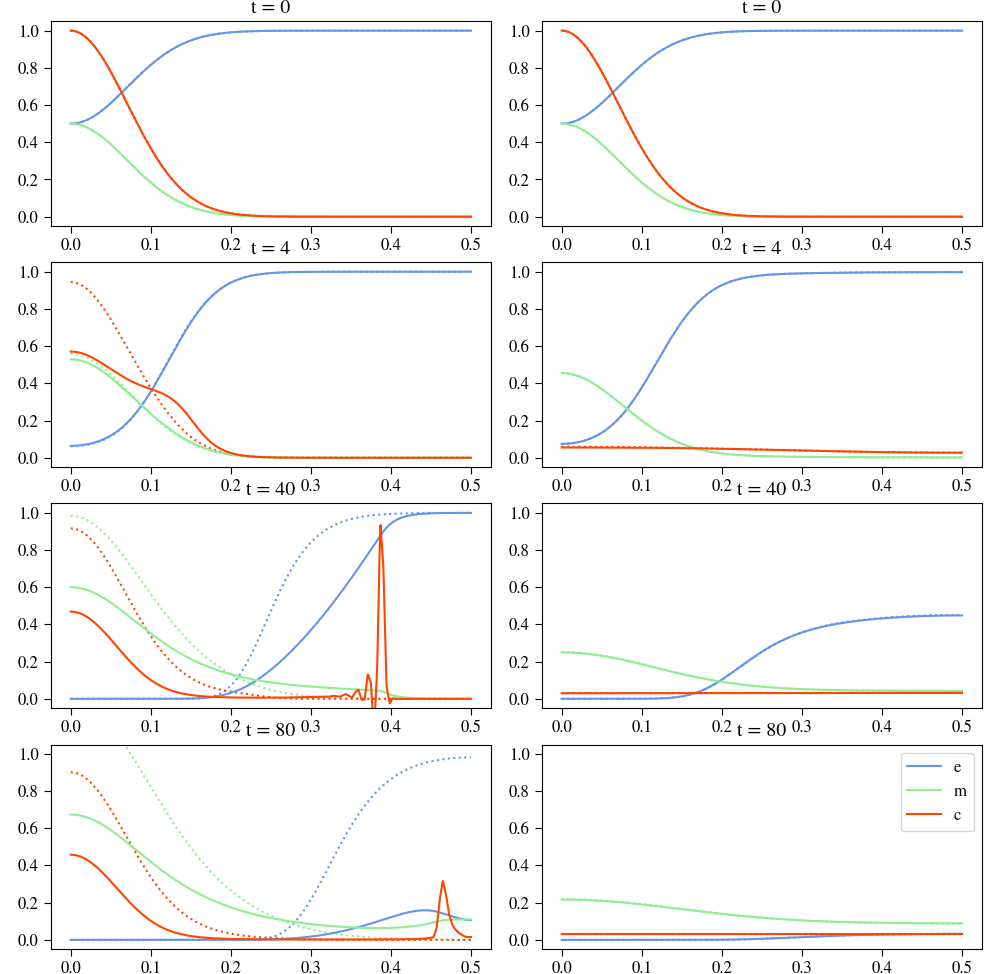
\includegraphics[width=0.85\textwidth]{resources/images/dc_gamma_variation.png}
    \caption{Plots show results for varying both $d_c$ and $\gamma$ whilst keeping the other parameters constant, in the images on the left $d_c$ is set to $d_c=5e-5$ with the solid line showing $\gamma = 0.01$ and the dotted line $\gamma=0.001$ on the right $d_c$ is set to $d_c=1e-1$ with the solid line showing $\gamma = 0.01$ and the dotted line $\gamma=0.001$.}
    \label{fig:dc_gamma_variation}
\end{figure}
lorem ipsum lorem ipsum lorem ipsum lorem ipsum lorem ipsum lorem ipsumlorem ipsum lorem ipsum lorem ipsum lorem ipsum lorem ipsum lorem ipsum lorem ipsumlorem ipsumlorem ipsum lorem ipsum lorem ipsum lorem ipsum lorem ipsum lorem ipsumlorem ipsumlorem ipsum lorem ipsum lorem ipsum lorem ipsum lorem ipsum lorem ipsumlorem ipsumlorem ipsum lorem ipsum lorem ipsum lorem ipsum lorem ipsum lorem ipsumlorem ipsumlorem ipsum lorem ipsum lorem ipsum lorem ipsum lorem ipsum lorem ipsumlorem ipsum lorem ipsum lorem ipsum lorem ipsum lorem ipsum lorem ipsum lorem ipsumlorem ipsum lorem ipsum lorem ipsum lorem ipsum lorem ipsum lorem ipsum lorem ipsumlorem ipsumlorem ipsum lorem ipsum lorem ipsum lorem ipsum lorem ipsum lorem ipsumlorem ipsumlorem ipsum lorem ipsum lorem ipsum lorem ipsum lorem ipsum lorem ipsumlorem ipsumlorem ipsum lorem ipsum lorem ipsum lorem ipsum lorem ipsum lorem ipsumlorem ipsumlorem ipsum lorem ipsum lorem ipsum lorem ipsum lorem ipsum lorem ipsumlorem ipsumlorem ipsum lorem ipsum lorem ipsum lorem ipsum lorem ipsum lorem ipsumlorem ipsum lorem ipsum lorem ipsum lorem ipsum lorem ipsum lorem ipsum lorem ipsumlorem ipsumlorem ipsum lorem ipsum lorem ipsum lorem ipsum lorem ipsum lorem ipsumlorem ipsumlorem ipsum lorem ipsum lorem ipsum lorem ipsum lorem ipsum lorem ipsumlorem ipsumlorem ipsum lorem ipsum lorem ipsum lorem ipsum lorem ipsum lorem ipsumlorem ipsumlorem ipsum lorem ipsum lorem ipsum lorem ipsum lorem ipsum lorem ipsumlorem ipsumlorem ipsum lorem ipsum lorem ipsum lorem ipsum lorem ipsum lorem ipsumlorem ipsum lorem ipsum lorem ipsum lorem ipsum lorem ipsum lorem ipsum lorem ipsumlorem ipsumlorem ipsum lorem ipsum lorem ipsum lorem ipsum lorem ipsum lorem ipsumlorem ipsumlorem ipsum lorem ipsum lorem ipsum lorem ipsum lorem ipsum lorem ipsumlorem ipsumlorem ipsum lorem ipsum lorem ipsum lorem ipsum lorem ipsum lorem ipsumlorem ipsumlorem ipsum lorem ipsum lorem ipsum lorem ipsum lorem ipsum lorem ipsumlorem ipsumlorem ipsum lorem ipsum lorem ipsum lorem ipsum lorem ipsum lorem ipsumlorem ipsum lorem ipsum lorem ipsum lorem ipsum lorem ipsum lorem ipsum lorem ipsumlorem ipsumlorem ipsum lorem ipsum lorem ipsum lorem ipsum lorem ipsum lorem ipsumlorem ipsumlorem ipsum lorem ipsum lorem ipsum lorem ipsum lorem ipsum lorem ipsumlorem ipsumlorem ipsum lorem ipsum lorem ipsum lorem ipsum lorem ipsum lorem ipsumlorem ipsumlorem ipsum lorem ipsum lorem ipsum lorem ipsum lorem ipsum lorem ipsumlorem ipsumlorem ipsum lorem ipsum lorem ipsum lorem ipsum lorem ipsum lorem ipsumlorem ipsum lorem ipsum lorem ipsum lorem ipsum lorem ipsum lorem ipsum lorem ipsumlorem ipsumlorem ipsum lorem ipsum lorem ipsum lorem ipsum lorem ipsum lorem ipsumlorem ipsumlorem ipsum lorem ipsum lorem ipsum lorem ipsum lorem ipsum lorem ipsumlorem ipsumlorem ipsum lorem ipsum lorem ipsum lorem ipsum lorem ipsum lorem ipsumlorem ipsumlorem ipsum lorem ipsum lorem ipsum lorem ipsum lorem ipsum lorem ipsumlorem ipsum

\subsubsection*{$d_m - \eta$ Variation}
\begin{figure}[h]
    \centering
    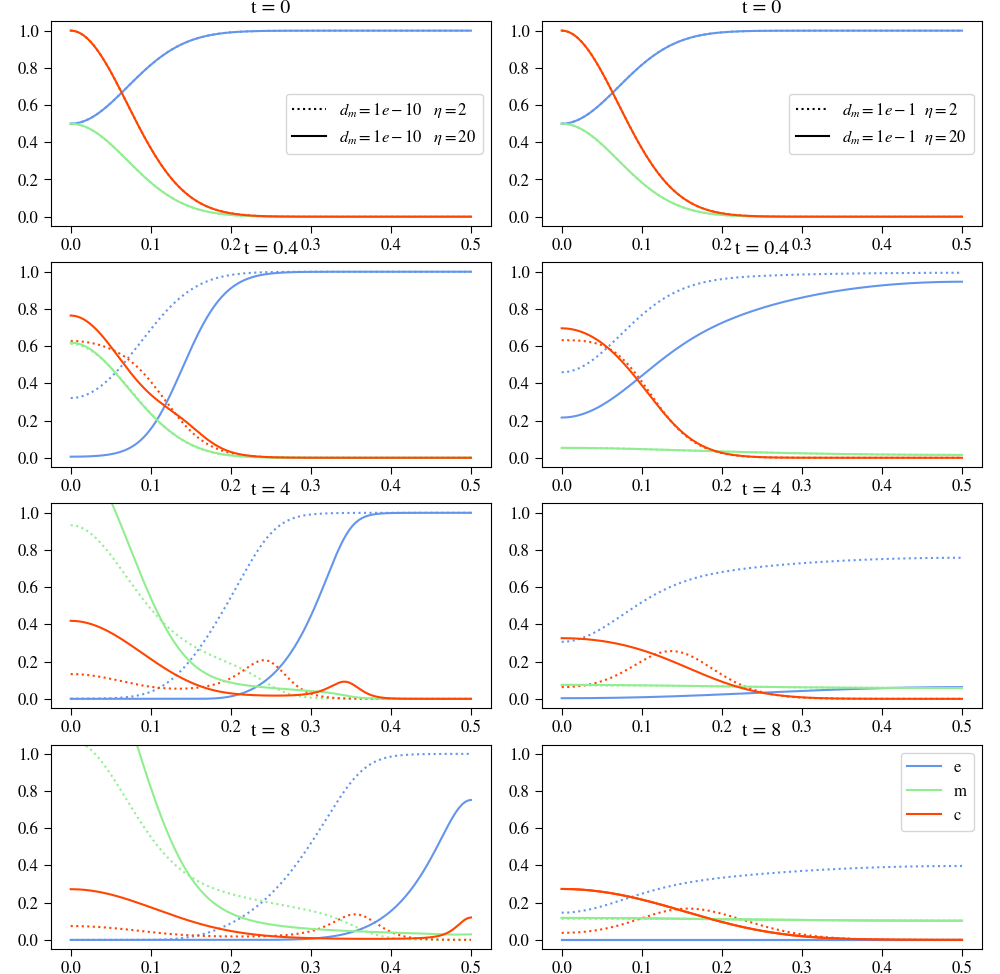
\includegraphics[width=0.85\textwidth]{resources/images/dm_eta_variation.png}
    \caption{Plots show results for varying both $d_m$ and $\eta$ whilst keeping the other parameters constant, in the images on the left $d_m$ is set to $d_c=1e-10$ with the solid line showing $\eta = 2$ and the dotted line $\eta=20$ on the right $d_m$ is set to $d_m=1e-1$ with the solid line showing $\eta = 2$ and the dotted line $\eta=20$.}
    \label{fig:dm_eta_variation}
\end{figure}
lorem ipsum lorem ipsum lorem ipsum lorem ipsum lorem ipsum lorem ipsumlorem ipsum lorem ipsum lorem ipsum lorem ipsum lorem ipsum lorem ipsum lorem ipsumlorem ipsumlorem ipsum lorem ipsum lorem ipsum lorem ipsum lorem ipsum lorem ipsumlorem ipsumlorem ipsum lorem ipsum lorem ipsum lorem ipsum lorem ipsum lorem ipsumlorem ipsumlorem ipsum lorem ipsum lorem ipsum lorem ipsum lorem ipsum lorem ipsumlorem ipsumlorem ipsum lorem ipsum lorem ipsum lorem ipsum lorem ipsum lorem ipsumlorem ipsum lorem ipsum lorem ipsum lorem ipsum lorem ipsum lorem ipsum lorem ipsumlorem ipsum lorem ipsum lorem ipsum lorem ipsum lorem ipsum lorem ipsum lorem ipsumlorem ipsumlorem ipsum lorem ipsum lorem ipsum lorem ipsum lorem ipsum lorem ipsumlorem ipsumlorem ipsum lorem ipsum lorem ipsum lorem ipsum lorem ipsum lorem ipsumlorem ipsumlorem ipsum lorem ipsum lorem ipsum lorem ipsum lorem ipsum lorem ipsumlorem ipsumlorem ipsum lorem ipsum lorem ipsum lorem ipsum lorem ipsum lorem ipsumlorem ipsumlorem ipsum lorem ipsum lorem ipsum lorem ipsum lorem ipsum lorem ipsumlorem ipsum lorem ipsum lorem ipsum lorem ipsum lorem ipsum lorem ipsum lorem ipsumlorem ipsumlorem ipsum lorem ipsum lorem ipsum lorem ipsum lorem ipsum lorem ipsumlorem ipsumlorem ipsum lorem ipsum lorem ipsum lorem ipsum lorem ipsum lorem ipsumlorem ipsumlorem ipsum lorem ipsum lorem ipsum lorem ipsum lorem ipsum lorem ipsumlorem ipsumlorem ipsum lorem ipsum lorem ipsum lorem ipsum lorem ipsum lorem ipsumlorem ipsumlorem ipsum lorem ipsum lorem ipsum lorem ipsum lorem ipsum lorem ipsumlorem ipsum lorem ipsum lorem ipsum lorem ipsum lorem ipsum lorem ipsum lorem ipsumlorem ipsumlorem ipsum lorem ipsum lorem ipsum lorem ipsum lorem ipsum lorem ipsumlorem ipsumlorem ipsum lorem ipsum lorem ipsum lorem ipsum lorem ipsum lorem ipsumlorem ipsumlorem ipsum lorem ipsum lorem ipsum lorem ipsum lorem ipsum lorem ipsumlorem ipsumlorem ipsum lorem ipsum lorem ipsum lorem ipsum lorem ipsum lorem ipsumlorem ipsumlorem ipsum lorem ipsum lorem ipsum lorem ipsum lorem ipsum lorem ipsumlorem ipsum lorem ipsum lorem ipsum lorem ipsum lorem ipsum lorem ipsum lorem ipsumlorem ipsumlorem ipsum lorem ipsum lorem ipsum lorem ipsum lorem ipsum lorem ipsumlorem ipsumlorem ipsum lorem ipsum lorem ipsum lorem ipsum lorem ipsum lorem ipsumlorem ipsumlorem ipsum lorem ipsum lorem ipsum lorem ipsum lorem ipsum lorem ipsumlorem ipsumlorem ipsum lorem ipsum lorem ipsum lorem ipsum lorem ipsum lorem ipsumlorem ipsumlorem ipsum lorem ipsum lorem ipsum lorem ipsum lorem ipsum lorem ipsumlorem ipsum lorem ipsum lorem ipsum lorem ipsum lorem ipsum lorem ipsum lorem ipsumlorem ipsumlorem ipsum lorem ipsum lorem ipsum lorem ipsum lorem ipsum lorem ipsumlorem ipsumlorem ipsum lorem ipsum lorem ipsum lorem ipsum lorem ipsum lorem ipsumlorem ipsumlorem ipsum lorem ipsum lorem ipsum lorem ipsum lorem ipsum lorem ipsumlorem ipsumlorem ipsum lorem ipsum lorem ipsum lorem ipsum lorem ipsum lorem ipsumlorem ipsum

\subsubsection*{$\alpha - \beta$ Variation}
\begin{figure}[h]
    \centering
    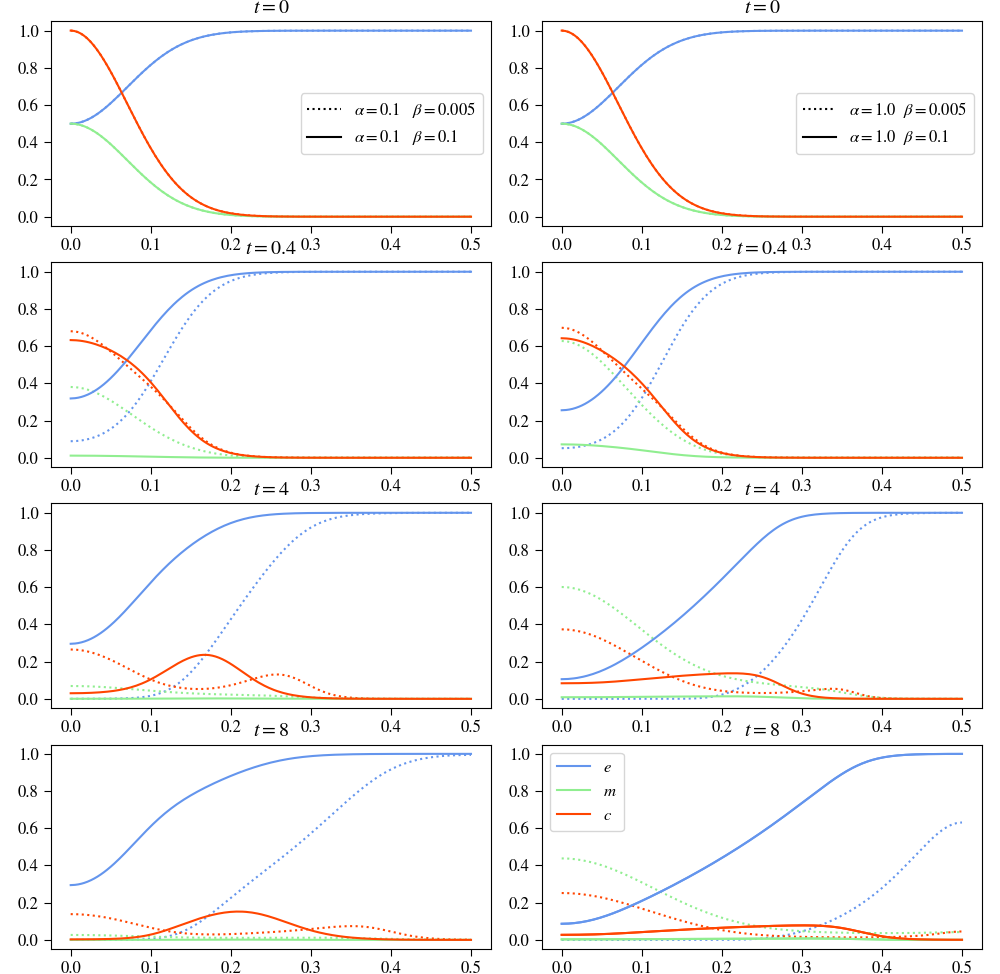
\includegraphics[width=0.85\textwidth]{resources/images/alpha_beta_variation.png}
    \caption{Plots show results for varying both $\alpha$ and $\beta$ whilst keeping the other parameters constant, in the images on the left $\alpha=0.1$ with the solid line showing $\beta = 0.005$ and the dotted line $\beta=0.1$ on the right $\alpha=1.0$ with the solid line showing $\beta = 0.005$ and the dotted line $\beta=0.1$.}
    \label{fig:alpha_beta_variation}
\end{figure}
lorem ipsum lorem ipsum lorem ipsum lorem ipsum lorem ipsum lorem ipsumlorem ipsum lorem ipsum lorem ipsum lorem ipsum lorem ipsum lorem ipsum lorem ipsumlorem ipsumlorem ipsum lorem ipsum lorem ipsum lorem ipsum lorem ipsum lorem ipsumlorem ipsumlorem ipsum lorem ipsum lorem ipsum lorem ipsum lorem ipsum lorem ipsumlorem ipsumlorem ipsum lorem ipsum lorem ipsum lorem ipsum lorem ipsum lorem ipsumlorem ipsumlorem ipsum lorem ipsum lorem ipsum lorem ipsum lorem ipsum lorem ipsumlorem ipsum lorem ipsum lorem ipsum lorem ipsum lorem ipsum lorem ipsum lorem ipsumlorem ipsum lorem ipsum lorem ipsum lorem ipsum lorem ipsum lorem ipsum lorem ipsumlorem ipsumlorem ipsum lorem ipsum lorem ipsum lorem ipsum lorem ipsum lorem ipsumlorem ipsumlorem ipsum lorem ipsum lorem ipsum lorem ipsum lorem ipsum lorem ipsumlorem ipsumlorem ipsum lorem ipsum lorem ipsum lorem ipsum lorem ipsum lorem ipsumlorem ipsumlorem ipsum lorem ipsum lorem ipsum lorem ipsum lorem ipsum lorem ipsumlorem ipsumlorem ipsum lorem ipsum lorem ipsum lorem ipsum lorem ipsum lorem ipsumlorem ipsum lorem ipsum lorem ipsum lorem ipsum lorem ipsum lorem ipsum lorem ipsumlorem ipsumlorem ipsum lorem ipsum lorem ipsum lorem ipsum lorem ipsum lorem ipsumlorem ipsumlorem ipsum lorem ipsum lorem ipsum lorem ipsum lorem ipsum lorem ipsumlorem ipsumlorem ipsum lorem ipsum lorem ipsum lorem ipsum lorem ipsum lorem ipsumlorem ipsumlorem ipsum lorem ipsum lorem ipsum lorem ipsum lorem ipsum lorem ipsumlorem ipsumlorem ipsum lorem ipsum lorem ipsum lorem ipsum lorem ipsum lorem ipsumlorem ipsum lorem ipsum lorem ipsum lorem ipsum lorem ipsum lorem ipsum lorem ipsumlorem ipsumlorem ipsum lorem ipsum lorem ipsum lorem ipsum lorem ipsum lorem ipsumlorem ipsumlorem ipsum lorem ipsum lorem ipsum lorem ipsum lorem ipsum lorem ipsumlorem ipsumlorem ipsum lorem ipsum lorem ipsum lorem ipsum lorem ipsum lorem ipsumlorem ipsumlorem ipsum lorem ipsum lorem ipsum lorem ipsum lorem ipsum lorem ipsumlorem ipsumlorem ipsum lorem ipsum lorem ipsum lorem ipsum lorem ipsum lorem ipsumlorem ipsum lorem ipsum lorem ipsum lorem ipsum lorem ipsum lorem ipsum lorem ipsumlorem ipsumlorem ipsum lorem ipsum lorem ipsum lorem ipsum lorem ipsum lorem ipsumlorem ipsumlorem ipsum lorem ipsum lorem ipsum lorem ipsum lorem ipsum lorem ipsumlorem ipsumlorem ipsum lorem ipsum lorem ipsum lorem ipsum lorem ipsum lorem ipsumlorem ipsumlorem ipsum lorem ipsum lorem ipsum lorem ipsum lorem ipsum lorem ipsumlorem ipsumlorem ipsum lorem ipsum lorem ipsum lorem ipsum lorem ipsum lorem ipsumlorem ipsum lorem ipsum lorem ipsum lorem ipsum lorem ipsum lorem ipsum lorem ipsumlorem ipsumlorem ipsum lorem ipsum lorem ipsum lorem ipsum lorem ipsum lorem ipsumlorem ipsumlorem ipsum lorem ipsum lorem ipsum lorem ipsum lorem ipsum lorem ipsumlorem ipsumlorem ipsum lorem ipsum lorem ipsum lorem ipsum lorem ipsum lorem ipsumlorem ipsumlorem ipsum lorem ipsum lorem ipsum lorem ipsum lorem ipsum lorem ipsumlorem ipsum


\subsubsection*{$d_m - \alpha - \beta$ Variation}
\begin{figure}[h]
    \centering
    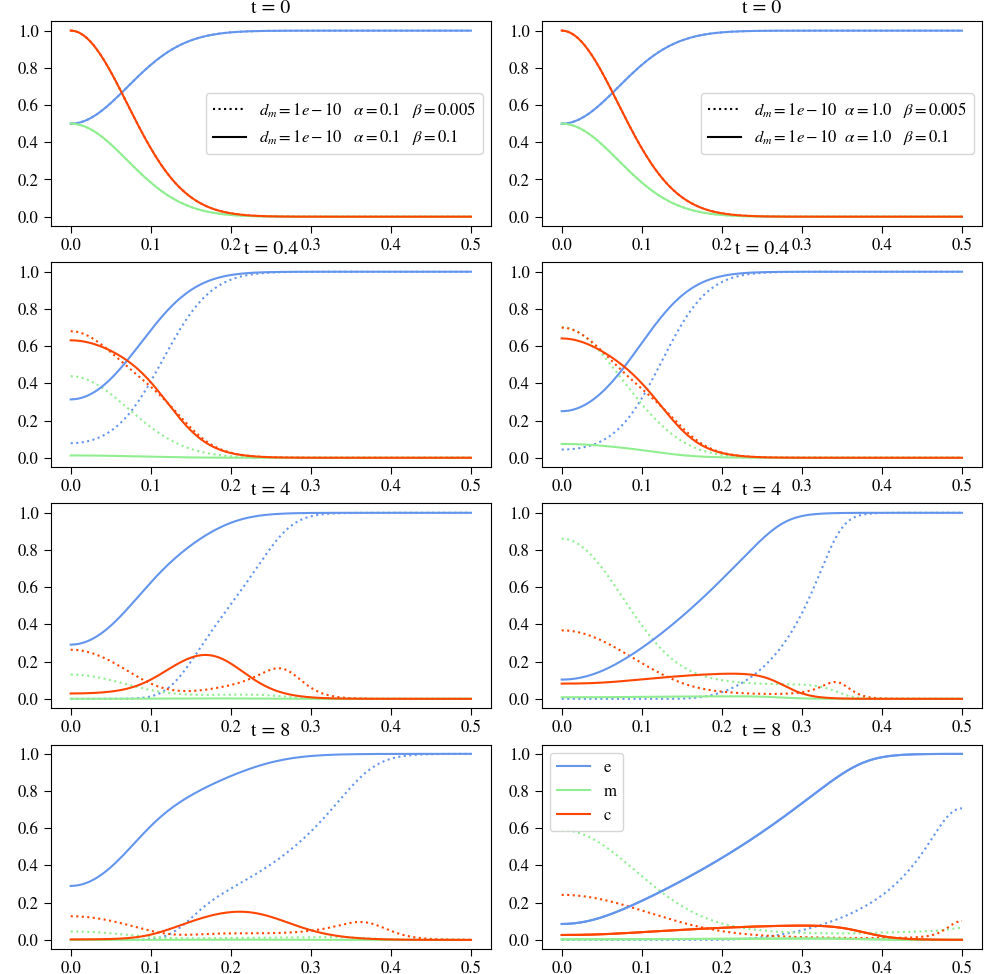
\includegraphics[width=0.85\textwidth]{resources/images/dm_alpha_beta_variation_1.png}
    \caption{Plots show results for varying both $\alpha$ and $\beta$ whilst keeping the other parameters constant, in the images on the left $\alpha=0.1$ with the solid line showing $\beta = 0.005$ and the dotted line $\beta=0.1$ on the right $\alpha=1.0$ with the solid line showing $\beta = 0.005$ and the dotted line $\beta=0.1$.}
    \label{fig:alpha_beta_variation}
\end{figure}
\begin{figure}[h]
    \centering
    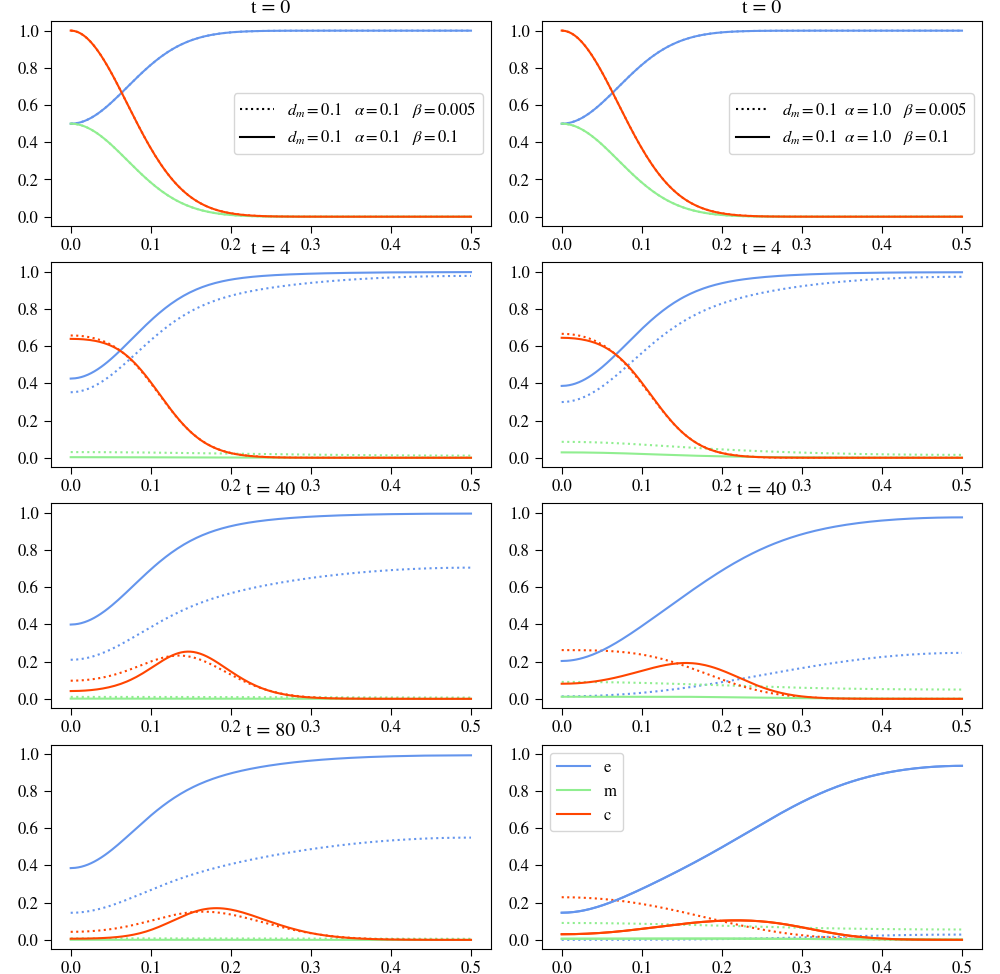
\includegraphics[width=0.85\textwidth]{resources/images/dm_alpha_beta_variation_2.png}
    \caption{Plots show results for varying both $\alpha$ and $\beta$ whilst keeping the other parameters constant, in the images on the left $\alpha=0.1$ with the solid line showing $\beta = 0.005$ and the dotted line $\beta=0.1$ on the right $\alpha=1.0$ with the solid line showing $\beta = 0.005$ and the dotted line $\beta=0.1$.}
    \label{fig:alpha_beta_variation}
\end{figure}
lorem ipsum lorem ipsum lorem ipsum lorem ipsum lorem ipsum lorem ipsumlorem ipsum lorem ipsum lorem ipsum lorem ipsum lorem ipsum lorem ipsum lorem ipsumlorem ipsumlorem ipsum lorem ipsum lorem ipsum lorem ipsum lorem ipsum lorem ipsumlorem ipsumlorem ipsum lorem ipsum lorem ipsum lorem ipsum lorem ipsum lorem ipsumlorem ipsumlorem ipsum lorem ipsum lorem ipsum lorem ipsum lorem ipsum lorem ipsumlorem ipsumlorem ipsum lorem ipsum lorem ipsum lorem ipsum lorem ipsum lorem ipsumlorem ipsum lorem ipsum lorem ipsum lorem ipsum lorem ipsum lorem ipsum lorem ipsumlorem ipsum lorem ipsum lorem ipsum lorem ipsum lorem ipsum lorem ipsum lorem ipsumlorem ipsumlorem ipsum lorem ipsum lorem ipsum lorem ipsum lorem ipsum lorem ipsumlorem ipsumlorem ipsum lorem ipsum lorem ipsum lorem ipsum lorem ipsum lorem ipsumlorem ipsumlorem ipsum lorem ipsum lorem ipsum lorem ipsum lorem ipsum lorem ipsumlorem ipsumlorem ipsum lorem ipsum lorem ipsum lorem ipsum lorem ipsum lorem ipsumlorem ipsumlorem ipsum lorem ipsum lorem ipsum lorem ipsum lorem ipsum lorem ipsumlorem ipsum lorem ipsum lorem ipsum lorem ipsum lorem ipsum lorem ipsum lorem ipsumlorem ipsumlorem ipsum lorem ipsum lorem ipsum lorem ipsum lorem ipsum lorem ipsumlorem ipsumlorem ipsum lorem ipsum lorem ipsum lorem ipsum lorem ipsum lorem ipsumlorem ipsumlorem ipsum lorem ipsum lorem ipsum lorem ipsum lorem ipsum lorem ipsumlorem ipsumlorem ipsum lorem ipsum lorem ipsum lorem ipsum lorem ipsum lorem ipsumlorem ipsumlorem ipsum lorem ipsum lorem ipsum lorem ipsum lorem ipsum lorem ipsumlorem ipsum lorem ipsum lorem ipsum lorem ipsum lorem ipsum lorem ipsum lorem ipsumlorem ipsumlorem ipsum lorem ipsum lorem ipsum lorem ipsum lorem ipsum lorem ipsumlorem ipsumlorem ipsum lorem ipsum lorem ipsum lorem ipsum lorem ipsum lorem ipsumlorem ipsumlorem ipsum lorem ipsum lorem ipsum lorem ipsum lorem ipsum lorem ipsumlorem ipsumlorem ipsum lorem ipsum lorem ipsum lorem ipsum lorem ipsum lorem ipsumlorem ipsumlorem ipsum lorem ipsum lorem ipsum lorem ipsum lorem ipsum lorem ipsumlorem ipsum lorem ipsum lorem ipsum lorem ipsum lorem ipsum lorem ipsum lorem ipsumlorem ipsumlorem ipsum lorem ipsum lorem ipsum lorem ipsum lorem ipsum lorem ipsumlorem ipsumlorem ipsum lorem ipsum lorem ipsum lorem ipsum lorem ipsum lorem ipsumlorem ipsumlorem ipsum lorem ipsum lorem ipsum lorem ipsum lorem ipsum lorem ipsumlorem ipsumlorem ipsum lorem ipsum lorem ipsum lorem ipsum lorem ipsum lorem ipsumlorem ipsumlorem ipsum lorem ipsum lorem ipsum lorem ipsum lorem ipsum lorem ipsumlorem ipsum lorem ipsum lorem ipsum lorem ipsum lorem ipsum lorem ipsum lorem ipsumlorem ipsumlorem ipsum lorem ipsum lorem ipsum lorem ipsum lorem ipsum lorem ipsumlorem ipsumlorem ipsum lorem ipsum lorem ipsum lorem ipsum lorem ipsum lorem ipsumlorem ipsumlorem ipsum lorem ipsum lorem ipsum lorem ipsum lorem ipsum lorem ipsumlorem ipsumlorem ipsum lorem ipsum lorem ipsum lorem ipsum lorem ipsum lorem ipsumlorem ipsum

\subsection{Two dimensional Results with Proliferation}


\subsubsection{Basecase Analysis}

\begin{figure}[h]
    \centering
    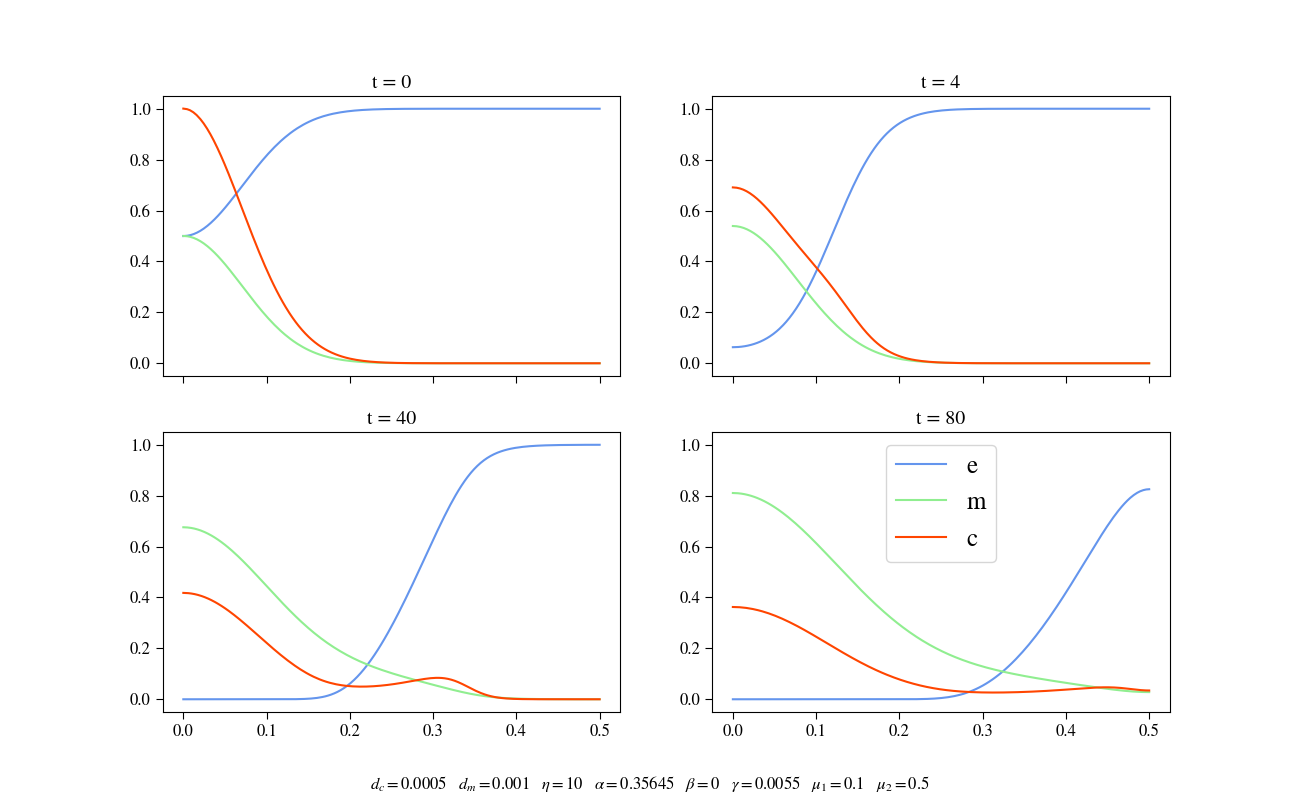
\includegraphics[width=\textwidth]{resources/images/basecase_proliferation.png}
    \label{fig:basecase_proliferation}
\end{figure}



\subsubsection{Parameter Analysis}

\subsubsection*{$d_c$ Variation}
% TODO: dc_variation schaubild einfuegen
\begin{figure}[h]
    \centering
    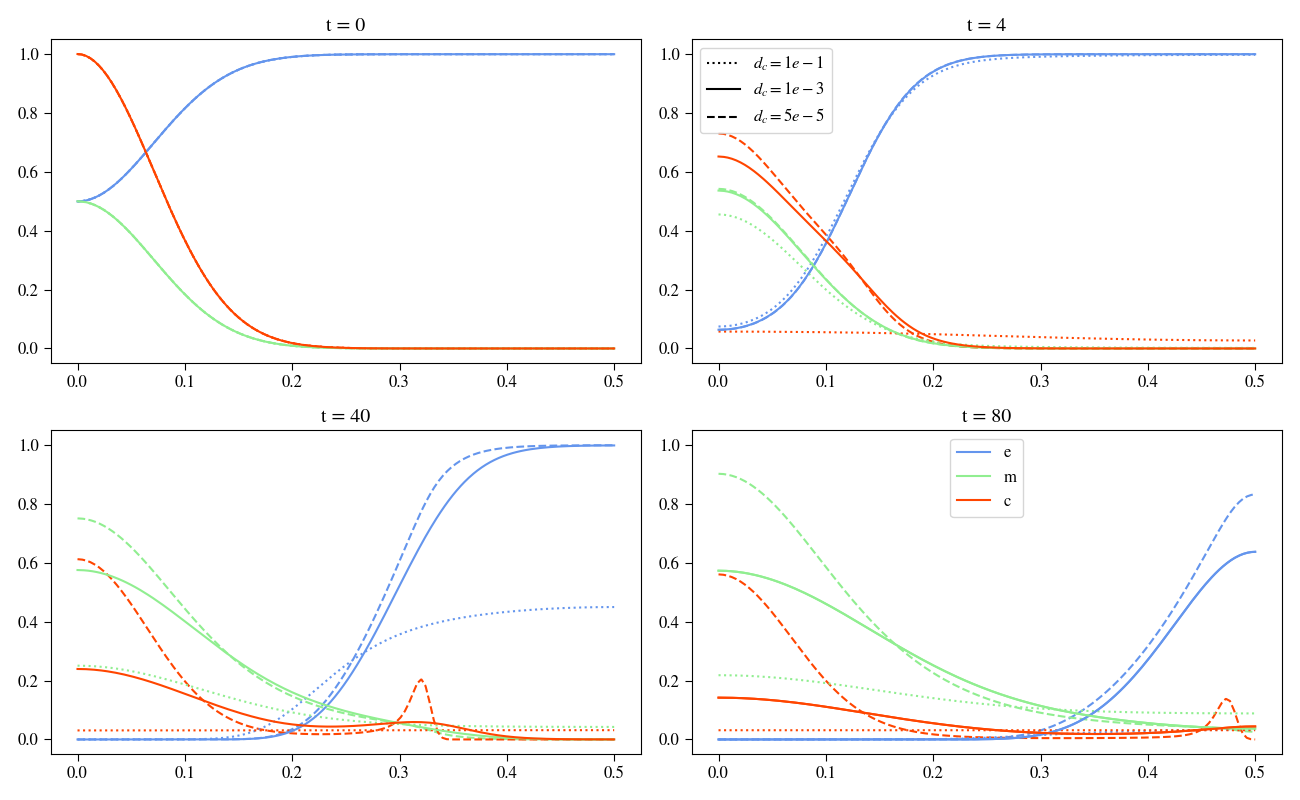
\includegraphics[width=\textwidth]{resources/images/dc_variation.png}
    \caption{Plots show results for varying $d_c$ whilst keeping the other parameters constant, in the images you can see the effects of $d_c=5e-5$ in the dashed curve, $d_c=1e-1$ in the dotted curve and $d_c=5e-4$ in the solid line.}
    \label{fig:dc_comparison}
\end{figure}


\subsubsection*{$\gamma$ Variation}

\begin{figure}[h]
    \centering
    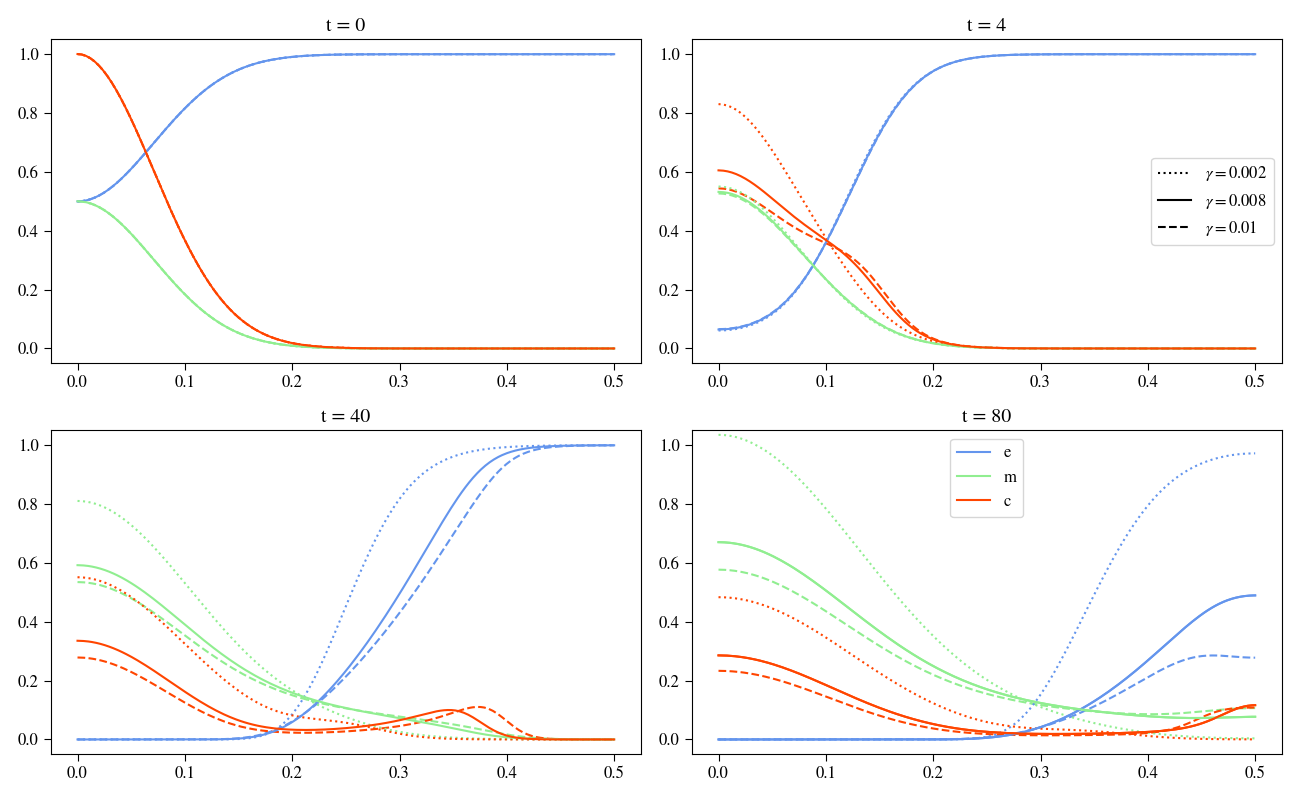
\includegraphics[width=\textwidth]{resources/images/prolif_gamma_variation.png}
    \caption{Plots show results for varying $\gamma$ whilst keeping the other parameters constant, in the images you can see the effects of $\gamma=0.01$ in the dashed curve, $\gamma=0.002$ in the dotted curve and $\gamma=0.008$ in the solid line.}
    \label{fig:gamma_variation}
\end{figure}


\subsubsection*{$\mu_1$ Variation}
% TODO:mu1 schaubild
\begin{figure}[h]
    \centering
    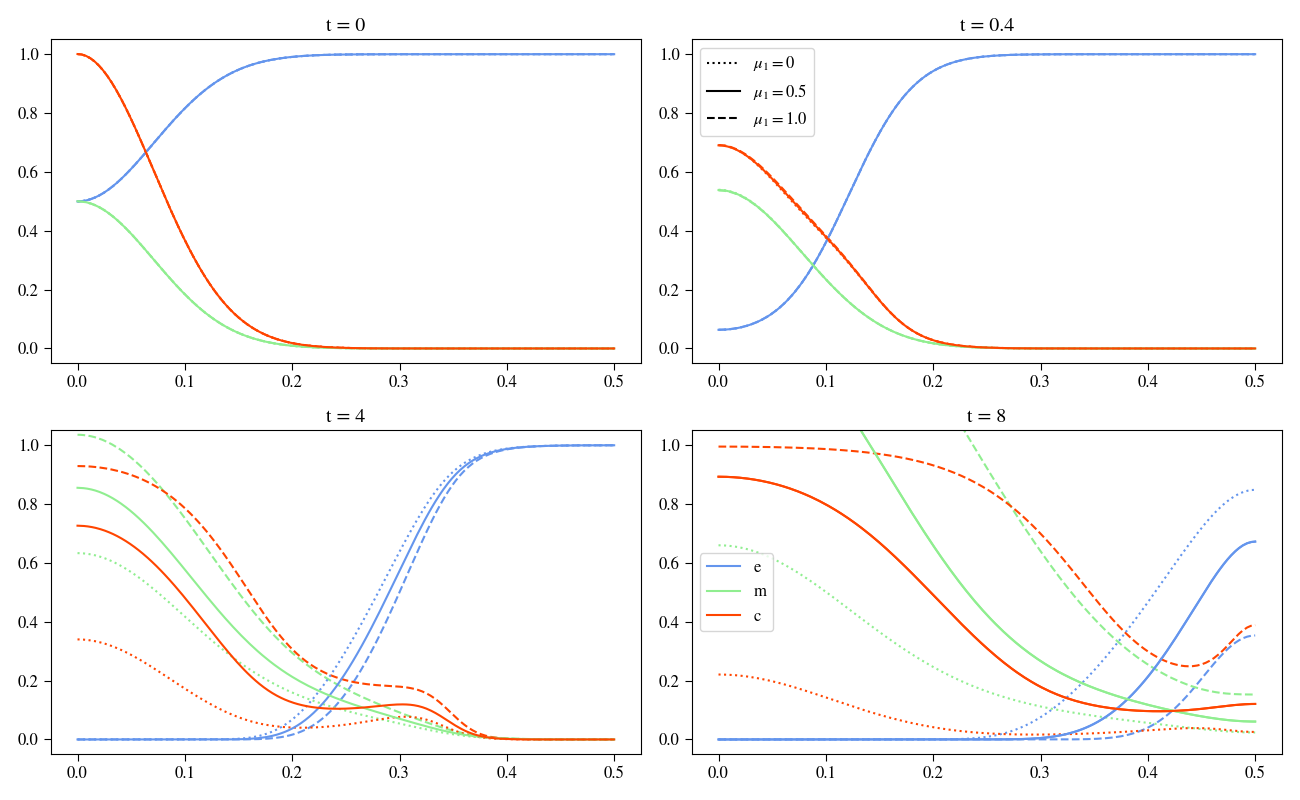
\includegraphics[width=\textwidth]{resources/images/prolif_mu_1_variation.png}
    \caption{Plots show results for varying $\eta$ whilst keeping the other parameters constant, in the images you can see the effects of $\eta=20$ in the dashed curve, $\eta=0$ in the dotted curve and $\eta=12$ in the solid line.}
    \label{fig:eta_variation}
\end{figure}


\subsubsection*{$\eta$ Variation}
\begin{figure}[h]
    \centering
    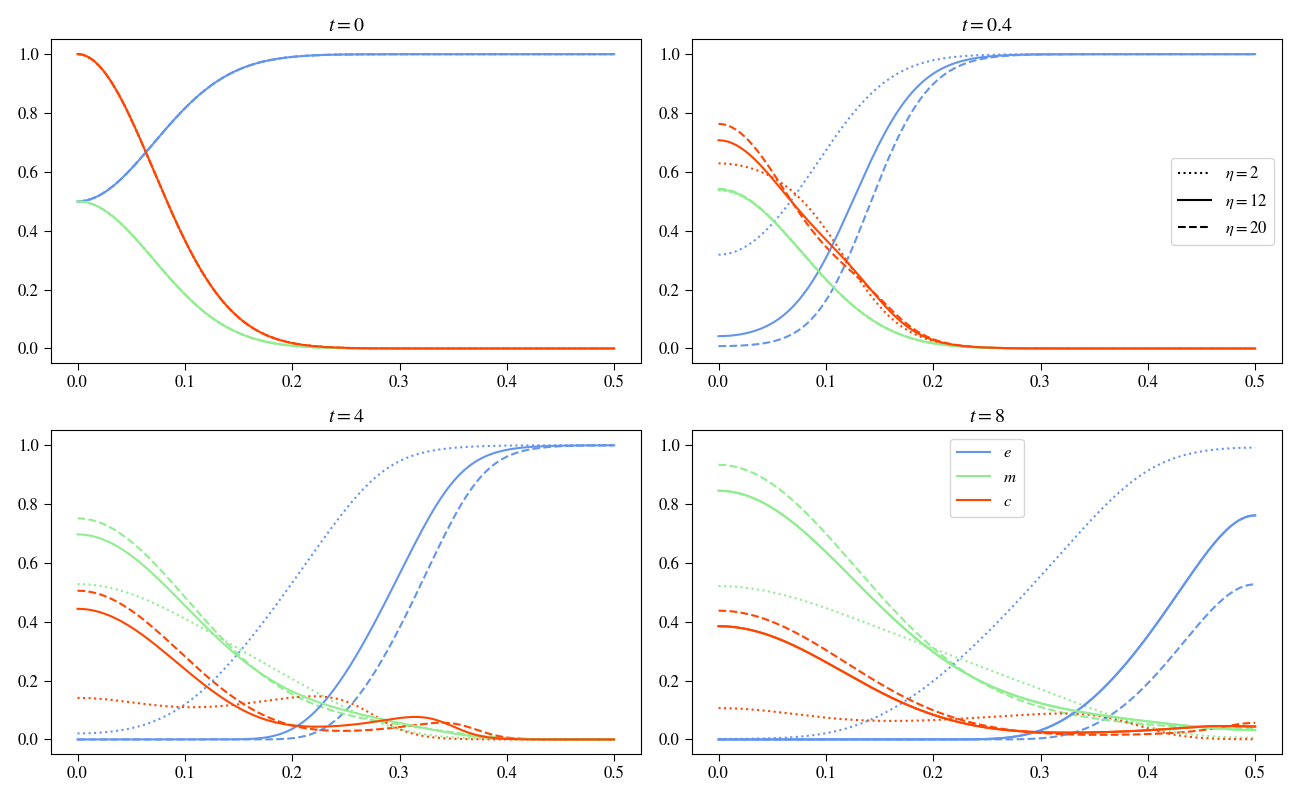
\includegraphics[width=\textwidth]{resources/images/prolif_eta_variation.png}
    \caption{Plots show results for varying $\eta$ whilst keeping the other parameters constant, in the images you can see the effects of $\eta=20$ in the dashed curve, $\eta=0$ in the dotted curve and $\eta=12$ in the solid line.}
    \label{fig:eta_variation}
\end{figure}


\subsubsection*{$\mu_2$ Variation}
\begin{figure}[h]
    \centering
    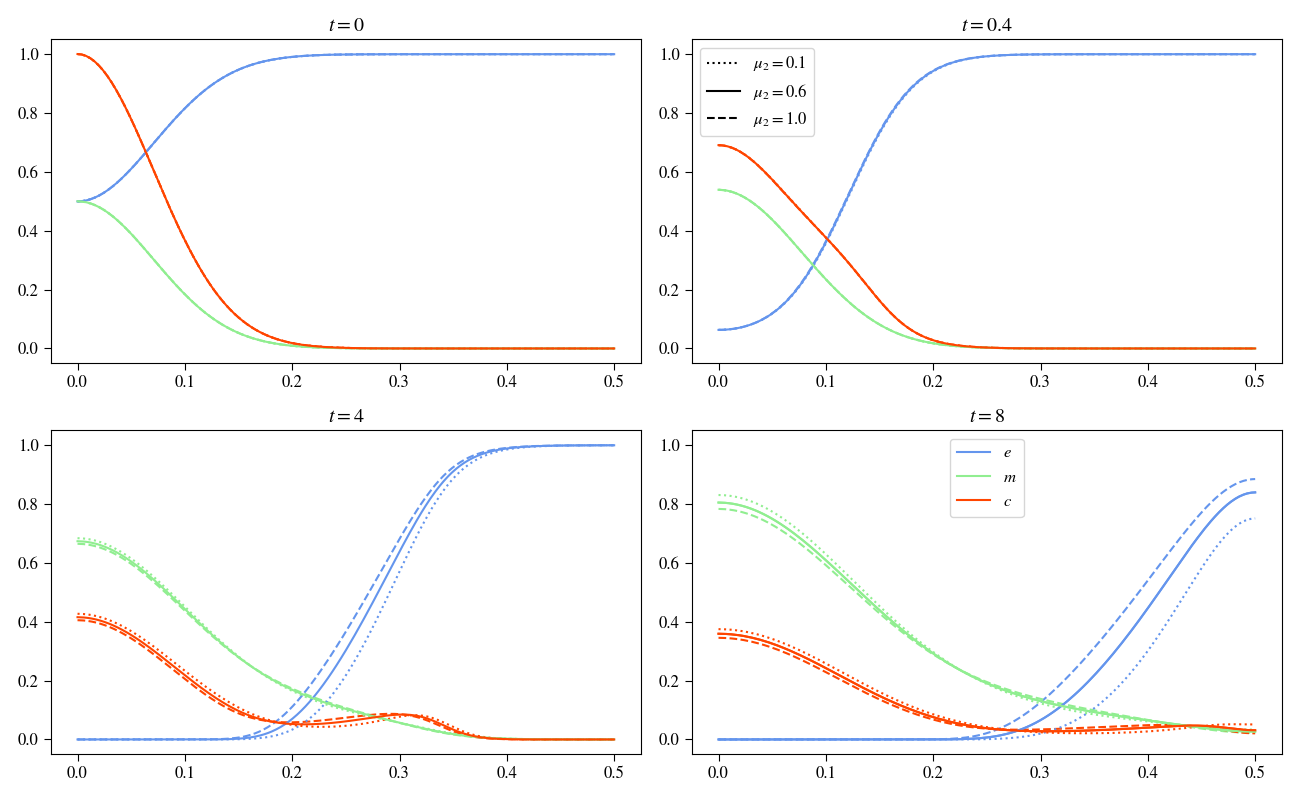
\includegraphics[width=\textwidth]{resources/images/prolif_mu_2_variation.png}
    \caption{Plots show results for varying $\eta$ whilst keeping the other parameters constant, in the images you can see the effects of $\eta=20$ in the dashed curve, $\eta=0$ in the dotted curve and $\eta=12$ in the solid line.}
    \label{fig:eta_variation}
\end{figure}

\subsubsection*{$d_m$ Variation}
%TODO: d_m Schaubild einfuegen
\begin{figure}[h]
    \centering
    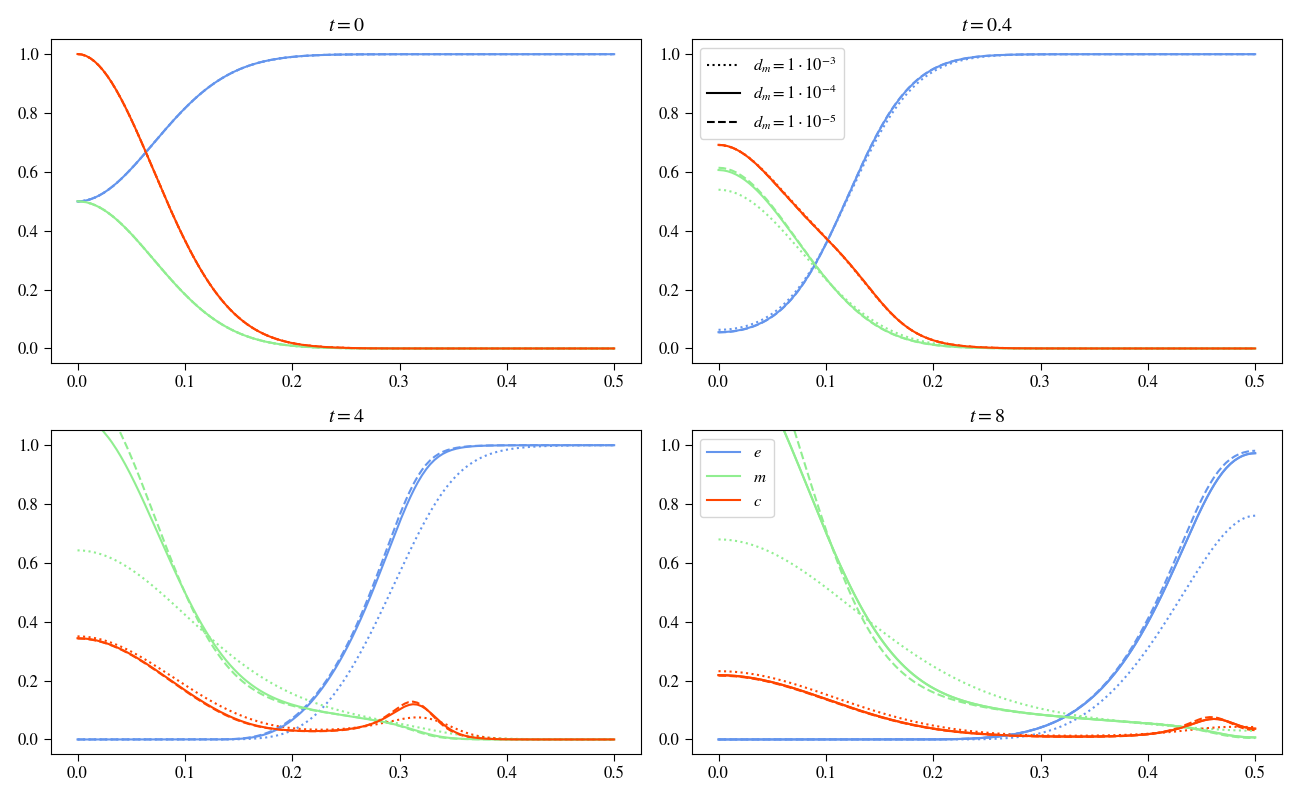
\includegraphics[width=\textwidth]{resources/images/dm_variation.png}
    \caption{Plots show results for varying $d_m$ whilst keeping the other parameters constant, in the images you can see the effects of $d_m=0.1$ in the dashed curve, $d_m=0$ in the dotted curve and $d_m=0.001$ in the solid line.}
    \label{fig:dm_variation}
\end{figure}

\subsubsection*{$\alpha$ Variation}
\begin{figure}[h]
    \centering
    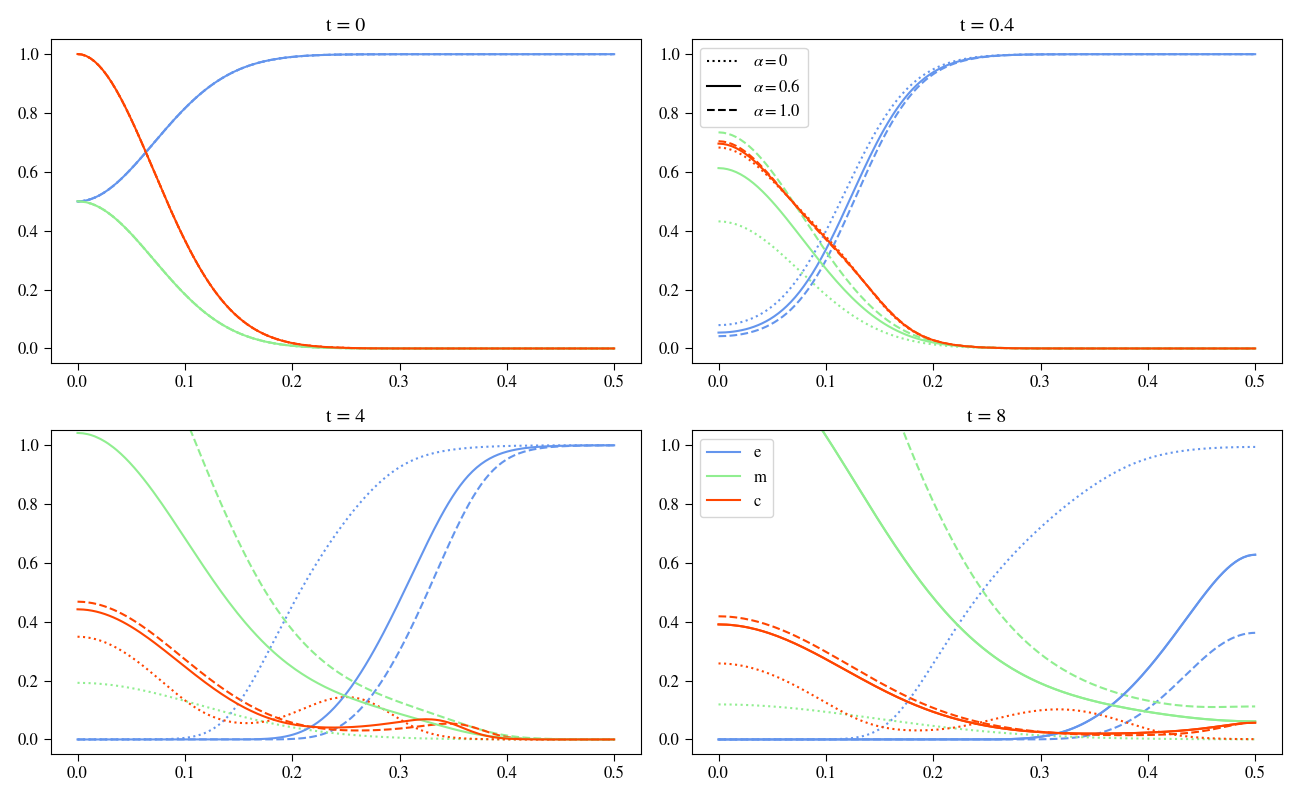
\includegraphics[width=\textwidth]{resources/images/prolif_alpha_variation.png}
    \caption{Plots show results for varying $\alpha$ whilst keeping the other parameters constant, in the images you can see the effects of $\alpha=1.0$ in the dashed curve, $\alpha=0$ in the dotted curve and $\alpha=0.6$ in the solid line.}
    \label{fig:alpha_variation}
\end{figure}

\subsubsection*{$\beta$ Variation}
\begin{figure}[h]
    \centering
    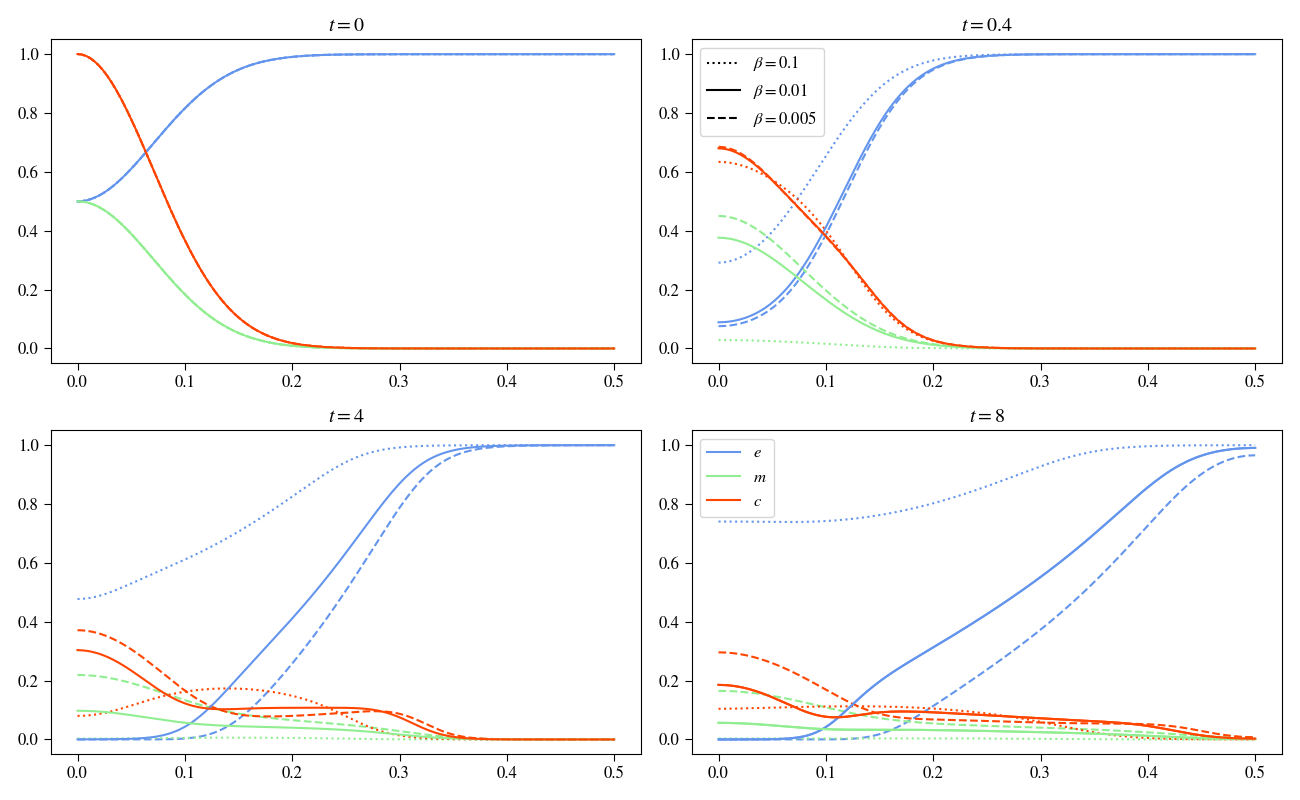
\includegraphics[width=\textwidth]{resources/images/prolif_beta_variation.png}
    \caption{Plots show results for varying $\beta$ whilst keeping the other parameters constant, in the images you can see the effects of $\beta=0.005$ in the dashed curve, $\beta=0.1$ in the dotted curve and $\beta=0.01$ in the solid line.}
    \label{fig:beta_variation}
\end{figure}

\subsubsection*{Cross Variation}

\subsubsection*{$d_c - \gamma - \mu_1$ Variation}
\begin{figure}[h]
    \centering
    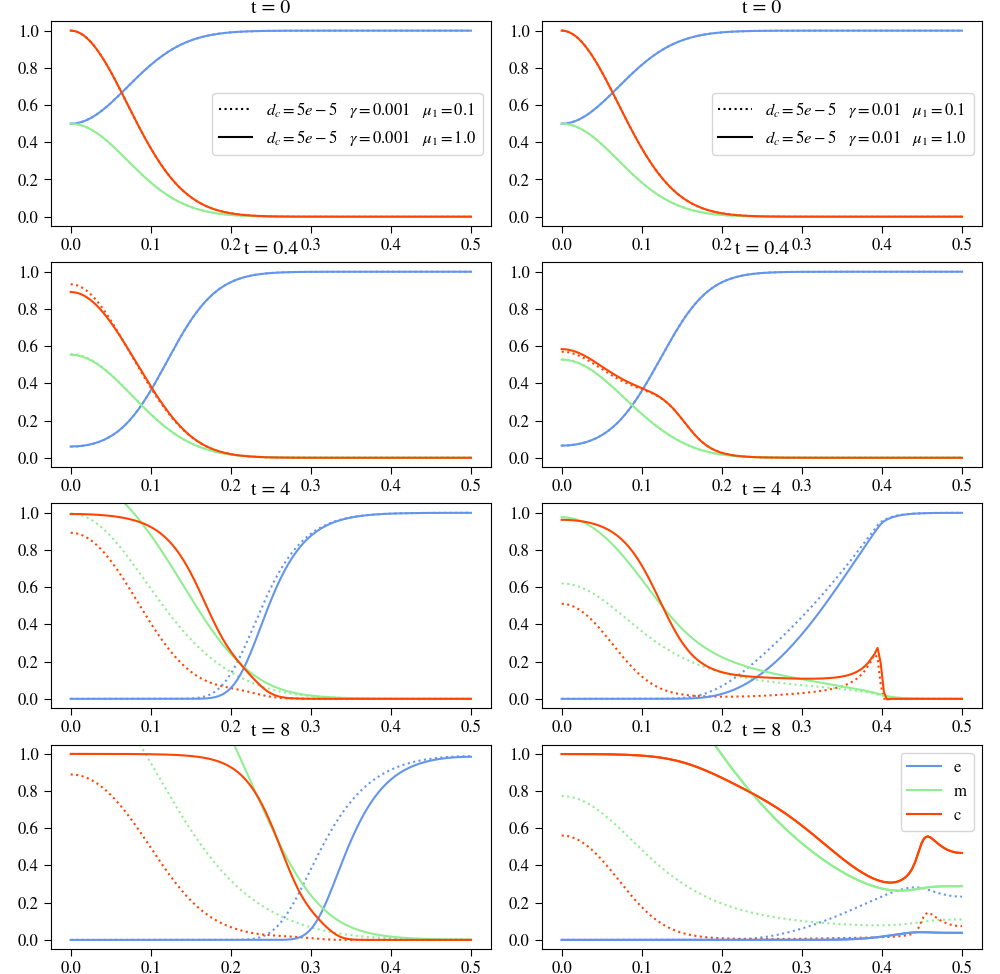
\includegraphics[width=0.85\textwidth]{resources/images/prolif_dc_gamma_mu1_1.png}
    \caption{Plots show results for varying both $d_c$ and $\gamma$ whilst keeping the other parameters constant, in the images on the left $d_c$ is set to $d_c=5e-5$ with the solid line showing $\gamma = 0.01$ and the dotted line $\gamma=0.001$ on the right $d_c$ is set to $d_c=1e-1$ with the solid line showing $\gamma = 0.01$ and the dotted line $\gamma=0.001$.}
    \label{fig:dc_gamma_variation}
\end{figure}

\begin{figure}[h]
    \centering
    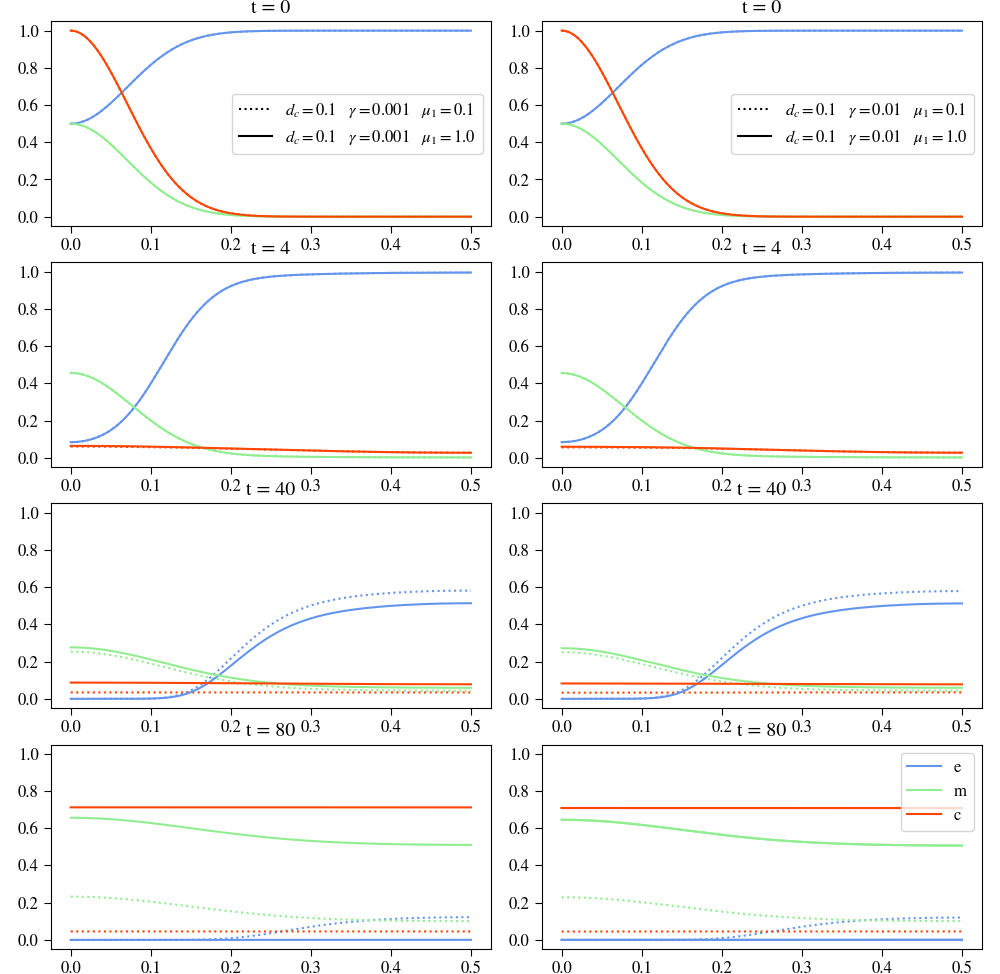
\includegraphics[width=0.85\textwidth]{resources/images/prolif_dc_gamma_mu1_2.png}
    \caption{Plots show results for varying both $d_c$ and $\gamma$ whilst keeping the other parameters constant, in the images on the left $d_c$ is set to $d_c=5e-5$ with the solid line showing $\gamma = 0.01$ and the dotted line $\gamma=0.001$ on the right $d_c$ is set to $d_c=1e-1$ with the solid line showing $\gamma = 0.01$ and the dotted line $\gamma=0.001$.}
    \label{fig:dc_gamma_variation}
\end{figure}

\subsubsection*{$\eta -\mu_2$ Variation}
\begin{figure}[h]
    \centering
    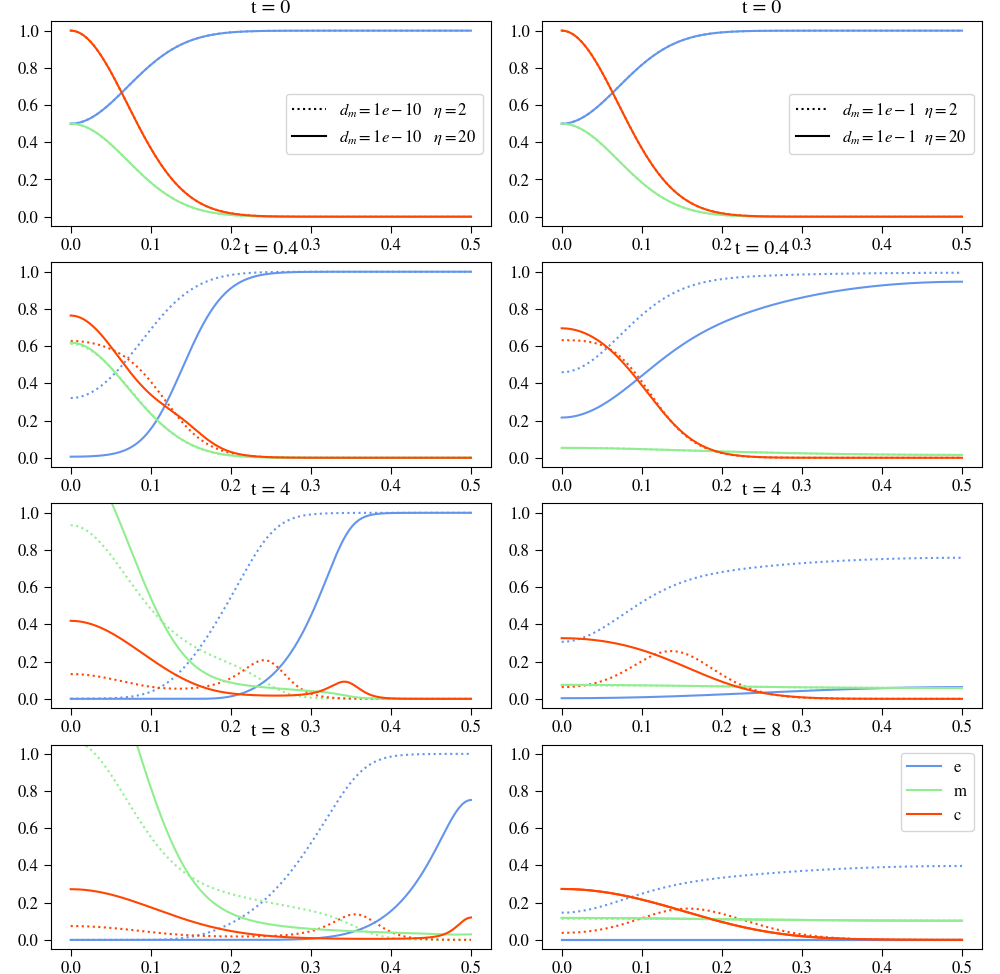
\includegraphics[width=0.85\textwidth]{resources/images/dm_eta_variation.png}
    \caption{Plots show results for varying both $d_m$ and $\eta$ whilst keeping the other parameters constant, in the images on the left $d_m$ is set to $d_c=1e-10$ with the solid line showing $\eta = 2$ and the dotted line $\eta=20$ on the right $d_m$ is set to $d_m=1e-1$ with the solid line showing $\eta = 2$ and the dotted line $\eta=20$.}
    \label{fig:dm_eta_variation}
\end{figure}






\subsection{Three Dimensional Results}
\subsubsection{Replicating Results}
\subsubsection{Parameter Analysis}
\subsection{Three Dimensional Simulations with Heterogenous ECM Structure}
